% Format teze zasnovan je na paketu memoir
% http://tug.ctan.org/macros/latex/contrib/memoir/memman.pdf ili
% http://texdoc.net/texmf-dist/doc/latex/memoir/memman.pdf
% 
% Prilikom zadavanja klase memoir, navedenim opcijama se podešava 
% veličina slova (12pt) i jednostrano štampanje (oneside).
% Ove parametre možete menjati samo ako pravite nezvanične verzije
% mastera za privatnu upotrebu (na primer, u b5 varijanti ima smisla 
% smanjiti 
\documentclass[12pt,oneside]{memoir} 

% Paket koji definiše sve specifičnosti master rada Matematičkog fakulteta
\usepackage[latinica]{matfmaster} 
\usepackage{elm-highlighting}
\usepackage{lmodern}
\usepackage{listings,xcolor}

\usepackage[T1]{fontenc}
\usepackage{xcolor}
\usepackage[scaled=0.9]{DejaVuSansMono}

\usepackage{multirow}
\usepackage{comment}

\lstdefinestyle{DOS}
{
    backgroundcolor=\color{black},
    basicstyle=\scriptsize\color{white}\ttfamily
}
\definecolor{commentgreen}{RGB}{2,112,10}
\definecolor{eminence}{RGB}{108,48,130}
\definecolor{weborange}{RGB}{255,165,0}
\definecolor{frenchplum}{RGB}{129,20,83}

\lstdefinelanguage{elixir}{
    morekeywords={case,catch,def,do,else,false,%
        use,alias,receive,timeout,defmacro,defp,%
        for,if,import,defmodule,defprotocol,%
        nil,defmacrop,defoverridable,defimpl,%
        super,fn,raise,true,try,end,with,field,type%
        unless, |>, <-, \}, \{, \%, ->},
 %   otherkeywords={->},
    sensitive=true,
    morecomment=[l]{\#},
    morecomment=[n]{/*}{*/},
    morecomment=[s][\color{purple}]{:}{\ },
    morestring=[s][\color{orange}]"",
    commentstyle=\color{commentgreen},
    keywordstyle=\color{eminence},
    stringstyle=\color{red},
	basicstyle=\ttfamily,
	breaklines,
	showstringspaces=false,
	frame=tb
}

%

%

%
% Opcija [biblatex]:
%   ako želite da koristite reference na više jezika i umesto paketa
%   bibtex da koristite BibLaTeX/Biber, dodajte opciju "biblatex" tj.
%   prethodni paket uključite pomoću: \usepackage[biblatex]{matfmaster}
%
% Opcija [b5paper]:
%   ako želite da napravite verziju teze u manjem (b5) formatu, navedite
%   opciju "b5paper", tj. prethodni paket uključite pomoću: 
%   \usepackage[b5paper]{matfmaster}. Tada ima smisla razmisliti o promeni
%   veličine slova (izmenom opcije 12pt na 11pt u \documentclass{memoir}).
%
% Naravno, opcije je moguće kombinovati.
% Npr. \usepackage[b5paper,biblatex]{matfmaster}


% Datoteka sa literaturom u BibTex tj. BibLaTeX/Biber formatu
\bib{matfmaster-primer}

% Ime kandidata na srpskom jeziku (u odabranom pismu)
\autor{Ana Petrović}
% Naslov teze na srpskom jeziku (u odabranom pismu)
\naslov{Testiranje softvera u funkcionalnim programskim jezicima Elm i Elixir}
% Godina u kojoj je teza predana komisiji
\godina{2023}
% Ime i afilijacija mentora (u odabranom pismu)
\mentor{dr Milena \textsc{Vujošević Janičić}, redovan profesor\\ Univerzitet u Beogradu, Matematički fakultet}
% Ime i afilijacija prvog člana komisije (u odabranom pismu)
\komisijaA{dr Filip \textsc{Marić}, vanredni profesor\\ Univerzitet u Beogradu, Matematički fakultet}
% Ime i afilijacija drugog člana komisije (u odabranom pismu)
\komisijaB{dr Ivan \textsc{Čukić}, docent\\ Univerzitet u Beogradu, Matematički fakultet}
% Ime i afilijacija trećeg člana komisije (opciono)
% \komisijaC{}
% Ime i afilijacija četvrtog člana komisije (opciono)
% \komisijaD{}
% Datum odbrane (odkomentarisati narednu liniju i upisati datum odbrane ako je poznat)
% \datumodbrane{}

% Apstrakt na srpskom jeziku (u odabranom pismu)
\apstr{%
Apstrakt
 % Quote: “Being proud of 100% test coverage is like being proud of reading every word in the newspaper. Some are more important than others.” - Kent Beck
}

% Ključne reči na srpskom jeziku (u odabranom pismu)
\kljucnereci{funkcionalno programiranje, testiranje, verifikacija softvera, programski jezik Elixir, programski jezik Elm}
% testiranje veb aplikacija? 

\begin{document}
% ==============================================================================
% Uvodni deo teze
\frontmatter
% ==============================================================================
% Naslovna strana
\naslovna
% Strana sa podacima o mentoru i članovima komisije
\komisija
% Strana sa posvetom (u odabranom pismu)
%\posveta{Mami, tati i dedi}
% Strana sa podacima o disertaciji na srpskom jeziku
\apstrakt
% Sadržaj teze
\tableofcontents*

% ==============================================================================
% Glavni deo teze
\mainmatter
% ==============================================================================

% ------------------------------------------------------------------------------
\chapter{Uvod}
% ------------------------------------------------------------------------------
\par
Ovde ide uvod .. ... ..... 
\par uvod uvod

\par sta se nalazi u kom poglavlju...


% ------------------------------------------------------------------------------
\chapter{Funkcionalna paradigma}
\label{chp:uvodnideo}

\par Funkcionalno programiranje je specifičan pristup programiranju, tj. programska paradigma, koja se zasniva na pojmu matematičke funkcije. Programi se kreiraju pomoću izraza i funkcija, bez izmena stanja i podataka \cite{func}. Iz tog razloga, jednostavniji su za razumevanje i otporniji na greške u odnosu na imperativne programe. Programski stil je deklarativnog tipa i umesto naredbi koriste se izrazi, tako da se izvršavanje programa svodi na evaluaciju izraza. Vrednost izraza je nezavisna od konteksta u kojem se izraz nalazi, što se naziva \emph{transparentnost referenci} i predstavlja osnovnu osobinu \emph{čistih} funkcionalnih jezika (eng. \textit{pure functional programming language}). Transparentnost referenci kao osnovnu posledicu ima nepostojanje propratnih efekata. Sa druge strane, \emph{nečisti} funkcionalni jezici (eng. \textit{impure functional programming language}) dozvoljavaju propratne efekte, koji mogu izazvati suptilne greške i biti teži za razumevanje. Međutim, praktičniji su za specifične vrste zadataka, kao što je programiranje korisničkog interfejsa ili rad sa bazom podataka. 
%\par Funkcionalni jezici zasnovani su na \textit{lambda računu} (eng. \textit{$\lambda$-calculus}), čija je osnovna svrha da d\a'a  definiciju izračunljivosti. Pored toga što se smatra prvim %funkcionalnim jezikom, lambda račun se naziva i najmanjim programskim jezikom na svetu. Sve što se može izračunati lambda računom smatra se izračunljivim. Ekspresivnost % funkcionalnih jezika ekvivalentna je ekspresivnosti Tjuringove mašine \cite{turing}. -- ova literatura je izbacena


\section{Karakteristike funkcionalnih jezika}
U nastavku su objašnjene neke od najvažnijih osobina jezika funkcionalne paradigme. 

\subsection{Funkcije kao građani prvog reda}
U funkcionalnim programima, funkcije se smatraju građanima prvog reda (eng. \emph{first class citizen}). To znači da u okviru jezika ne postoje restrikcije po pitanju njihovog kreiranja i korišćenja. Građani prvog reda su entiteti u okviru programskog jezika koji mogu biti:
\begin{itemize}
\item deo nekog izraza
\item dodeljeni nekoj promenljivoj
\item prosleđeni kao argument funkcije
\item povratne vrednosti funkcije
\end{itemize}
Mogućnost prosleđivanja funkcija kao argumenata drugih funkcija je ključna za funkcionalnu paradigmu. 

\subsection{Čista funkcija}
\par  Čista funkcija (eng. \textit{pure function}) ima dve osnovne karakteristike: 
\begin{itemize}
\item Transparentnost referenci 
\item Imutabilnost 
\end{itemize}
\par  Koncept transparetnosti referenci se odnosi na to da je vrednost izraza jedinstveno određena. Izraz se može zameniti svojom vrednošću na bilo kom mestu u programu, bez promene u ponašanju programa. Definicija se može proširiti i na funkcije: funkcija poseduje transparentnost referenci ako pri pozivu sa istim vrednostima argumenata uvek proizvodi isti rezultat. Ponašanje takve funkcije je određeno njenim ulaznim vrednostima.
\par Imutabilnost podrazumeva odsustvo propratnih efekata, tj. da čista funkcija ne vrši nikakve izmene nad argumentima, kao ni nad promenljivima. Jedini rezultat čiste funkcije jeste vrednost koju ona vrati. Kao posledica ovoga, funkcionalni programi su laki za debagovanje. Čiste funkcije takođe olakšavaju paralelizaciju i konkurentnost aplikacija. Na osnovu ovako napisanih programa, kompilator lako može da paralelizuje naredbe, sačeka da evaluira rezultate kada budu potrebni, i na kraju da zapamti rezultat, s obzirom na to da se on neće promeniti sve dok ulaz ostaje isti. K$\hat{o}$d \ref{lst:pure} prikazuje primer jedne čiste funkcije u programskom jeziku Elixir. 

\begin{lstlisting}[language=elixir, caption={Primer čiste funkcije},captionpos=b, label={lst:pure}]
defmodule Math do 
  def fibonacci(0) do 0 end
  def fibonacci(1) do 1 end
  def fibonacci(n) do fibonacci(n-1) + fibonacci(n-2) end
end

IO.puts Math.fibonacci(9)
\end{lstlisting}

\subsection{Funkcije višeg reda}
Funkcija višeg reda je funkcija koja kao argument uzima jednu ili više funkcija i/ili ima funkciju kao svoju povratnu vrednost. U funkcionalnom programiranju se intenzivno koriste ovakve funkcije, a po svojoj važnosti se posebno izdvajaju \textit{map}, \textit{filter} i \textit{reduce (fold)}.  Funkcija \textit{map} kao argumente prima funkciju i listu, i zatim primeni datu funkciju na svaki element liste i kao povratnu vrednost proizvodi novu listu. Upotrebom funkcije \textit{filter} mogu se eliminisati neželjeni elementi neke liste --- na osnovu prosleđene funkcije predikata i date liste, \textit{filter} vraća listu sa elementima koji ispunjavaju dati kriterijum. \textit{Fold} prihvata tri argumenta: funkciju spajanja, početnu vrednost i listu. Iznova primenjuje funkciju spajanja na početnu vrednost i datu listu, sve dok se rezultat ne redukuje na jednu vrednost. 
\par Prednost korišćenja ovih funkcija je u sažetom i čistom kodu. Takođe, pogodne su i za paralelizaciju. Primer koda \ref{lst:high} pokazuje upotrebu funkcija višeg reda u programskom jeziku Elm.


\begin{lstlisting}[language=elm, caption={Funkcije višeg reda},captionpos=b, label={lst:high}]
[1, 2, 3] |> List.map (\number -> number * 2) -- [2, 4, 6]
[1, 2, 3, 4, 5] |> List.filter (\number -> number <= 3) -- [1, 2, 3]
[1, 2, 3, 4, 5] |> List.foldl (\item total -> total + item) 0 -- 15
\end{lstlisting}

\subsection{Odsustvo promenljivih i rekurzija}
\par Čisti funkcionalni jezici nemaju stanje koje bi se menjalo tokom izvršavanja programa, pa zbog toga ne podržavaju koncept promenljivih. Sa druge strane, nečisti funkcionalni jezici podržavaju i karakteristike drugih programskih paradigmi, te je u okviru njih dozvoljena upotreba promenljivih. Iako su fleksibilniji po tom pitanju, nečisti funkcionalni jezici promovišu imutabilnost kao dobru praksu. 
\par Kod funkcionalno napisanih programa može se primetiti odsustvo petlji. Funkcije se definišu rekurzivno --- pozivaju same sebe i time postižu ponavljanje izvršavanja. U mnogim slučajevima, umesto rekurzije se koriste funkcije višeg reda.

\section{Testiranje u razvoju softvera}
\label{sec:piramid}

\par Testiranje koda je jedan od najvažnijih aspekata u procesu razvoja softvera. Cilj testiranja je pronalaženje grešaka, proverom da li su ispunjeni svi funkcionalni i nefunkcionalni zahtevi \cite{test}.  Softver koji ne radi onako kako je predviđeno može dovesti do različitih problema, kao što su gubitak novca i vremena, ili u najgorim slučajevima --- povrede ili smrti. Testiranjem se osigurava kvalitet softvera i smanjuje rizik od neželjenog ponašanja. Glavna uloga testiranja jeste verifikacija softvera --- provera da li sistem zadovoljava specifikaciju, ali uključuje i validaciju --- proveru da li sistem ispunjava sve potrebe korisnika.  

%\par Razvoj vođen testovima (eng. \emph{Test-Driven Development , TDD}) je praksa u razvoju softvera koja nalaže da se prvo napišu testovi. Ti testovi na početku ne prolaze, s obzirom na to da k$\hat{o}$d još uvek nije implementiran, a zatim se iznova pokreću tokom pisanja samog koda, sve dok ne prođu. Ova tehnika kontinualnog testiranja tokom razvoja se često preporučuje jer se lako i veoma rano uoče greške i time sprečavaju u kasnijim fazama razvoja. Ipak, u ovom radu neće biti primenjen TDD pristup. Kako je tema testiranje, fokus nije na pisanju koda aplikacije, već testova za već napisan projekat. Aplikacija koja će biti testirana služi samo kao primer na kome će biti prikazani značajni koncepti testiranja funkcionalnih programa. Kratak opis testiranog projekta biće preciznije objašnjen u poglavlju \ref{chp:msnr}. 

\subsection{Organizacija testova}
\par Model piramide testiranja (prikazan na slici \ref{fig:piramida}) je koncept koji pomaže u razmišljanju o tome kako testirati softver \cite{cohn}. Uloga piramide je da vizuelno predstavi logičku organizaciju standarda u testiranju. Sastoji se od tri sloja: bazu piramide predstavljaju jedinični testovi (eng. \emph{unit test}). Njih bi trebalo da bude najviše --- kako su najmanji, samim tim su i najbrži, a izvršavaju se u potpunoj izolaciji. Na sledećem nivou, u sredini piramide, nalaze se integracioni testovi. Integracija podrazumeva način na koji različite komponente sistema rade zajedno. Nisu potrebne interakcije sa korisničkim interfejsom, s obzirom na to da ovi testovi pozivaju k$\hat{o}$d preko interfejsa. Vrh piramide čine sistemski testovi. Oni se ne fokusiraju na individualne komponente, već testiraju čitav sistem kao celinu i time utvrđuju da on radi očekivano i ispunjava sve funkcionalne i nefunkcionalne zahteve. Takvi testovi su prilično skupi, pa je potrebno doneti odluku koliko, i koje od njih se isplati sprovesti.
\par Jedna vrsta sistemskih testova su takozvani E2E testovi\footnote{E2E je skraćenica za testove sa kraja na kraj (eng. \emph{end-to-end})}, koji simuliraju korisničko iskustvo kako bi osigurali da sistem funkcioniše kako treba, od korisničkog interfejsa, pa sve do serverske strane i baze podataka. Testovi korisničkog interfejsa (eng. \emph{User Interface tests, UI tests}) se staraju o tome da se korisnički interfejs ponaša na očekivan način. Obično su automatski i simuliraju interakcije pravih korisnika sa aplikacijom, kao što su pritiskanje dugmića, unos teksta i slično. S obzirom na to da oni proveraju da sistem, zajedno sa svojim korisničkim interfejsom, radi kako treba --- mogu se u određenom kontekstu smatrati sistemskim testovima, ali su ipak specifičniji i mogu se sprovoditi i nezavisno od celokupnog sistema. 
\par U opštem slučaju, testiranje projekta koji se sastoji od više slojeva podrazumeva kombinaciju jediničnih, integracionih i sistemskih testova kako bi se osigurala ukupna funcionalnost, pouzdanost i perfomanse sistema.

\begin{figure}[!ht]
  \centering
  \label{fig:piramida}
  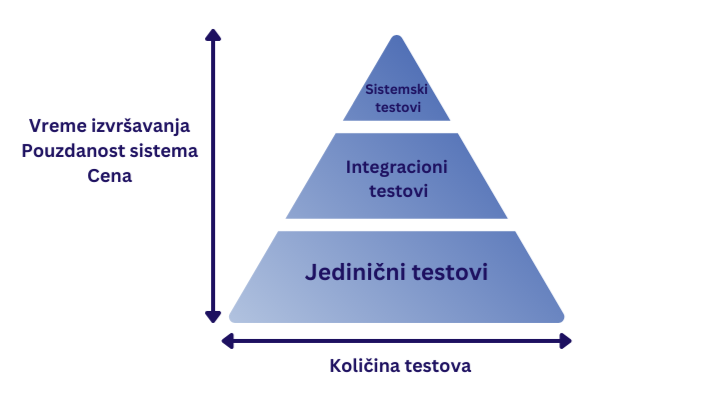
\includegraphics[width=0.8\textwidth]{piramidanova.png}
  \caption{Model piramide testiranja}
\end{figure}

\subsubsection{Anatomija testa}
\par Kako bi k$\hat{o}$d testa bio čitljiv i jednostavan za razumevanje, obrazac četvorofaznog testa (eng. \emph{four-phase test}) predlaže strukturu testa koja podrazumeva ne više od četiri faze \cite{4phase}. Svaki test se može podeliti na četiri jasno odvojive celine:  
\begin{enumerate}
\item Priprema (eng. \emph{setup}) --- sređivanje podataka koji će se prosleđivati pred samu proveru (uglavnom nije neophodno u testiranju čisto funkcionalnih programa).
\item Delovanje (eng. \emph{exercise}) --- pozivanje koda koji se testira, ključni deo svakog testa.
\item Verifikacija (eng. \emph{verify}) --- testovi proveravaju ponašanje koda (često se spaja sa prethodnom fazom). 
\item Rušenje (eng. \emph{teardown}) --- vraćanje podataka na prvobitno stanje, npr. ako se u prvoj fazi koriste neka deljena stanja, kao što je baza podataka. Ovaj korak se često izvršava implicitno. 
\end{enumerate}

\par Konkretan primer ovako organizovanog testa u programskom jeziku Elm dat je u primeru \ref{lst:4ph}. Definisan je jednostavan jedinični test, koji proverava da li funkcija koja sabira dva broja daje ispravan rezultat. U fazi pripreme brojevima i njihovoj očekivanoj sumi se dodeljuju vrednosti . U fazi delovanja poziva se funkcija \emph{sum}, a pozivanjem funkcije \emph{expect} proverava se da li je rezultat jednak očekivanom u fazi verifikacije. Faza rušenja u ovom slučaju ne treba da uradi ništa.

\begin{lstlisting}[language=elm, caption={Četiri faze jediničnog testa koji proverava ispravnost
funkcije sabiranja dva broja},captionpos=b, label={lst:4ph}]
import Test exposing (..)

sumTest : Test
sumTest =
    describe "sum" [
      test "should add two numbers correctly" <| \() -> 
        let
        --Setup
           x = 2
           y = 3
           expected = 5
        in
        -- Exercise (sum)
        -- Verify (expect)
           expect (sum x y) |> toEqual expected
    ]

   -- Teardown
   teardown : Int -> ()
   teardown _ =
    ()
\end{lstlisting}

\subsubsection{Testovi jedinica koda}
\par Jedinica je mala logička celina koda: može biti funkcija, klasa, metod klase, modul i slično. Jedinični test proverava samo da li se data jedinica ponaša prema svojoj specifikaciji. Ovi testovi se mogu pisati u potpunoj izolaciji, i ne zavise ni od jedne druge komponente, servisa, ni korisničkog interfejsa. Dakle, izdvajaju se najmanji testabilni delovi aplikacije i proverava se da li rade ono za šta su namenjeni. Ovi testovi su po pravilu najbrži i  najjednostavniji za pisanje jer se bave malim delom aplikacije, te je k$\hat{o}$d koji se testira najčešće vrlo jednostavan. 
\par Cilj jediničnih testova jeste da spreče greške koje mogu nastati izmenama koda, kao i da omoguće da se lako utvrdi lokacija dela koda koji izaziva grešku. Pri dizajniranju ovih testova, potrebno je proveriti da k$\hat{o}$d radi tačno ono za šta je namenjen, a da se to uradi pisanjem najmanje moguće dodatne količine koda.
\par Može se diskutovati o tome šta se smatra "jedinicom", a posebno u kontekstu funkcionalnog programiranja. Uobičajeno je da se jedinični testovi fokusiraju na pojedinačnu funkciju i njenu logiku, kako bi se opseg testa održavao što užim, radi bržeg pronalaženja grešaka. Međutim, nekada ima smisla da se u opseg testa uključi više modula ili procesa, i time se proširi definicija jedinice koda i olakša održavanje samih testova. 


\subsubsection{Integracioni testovi}
\label{sec:integration}
\par Jedan od ključnih koraka u razvoju softvera jeste pisanje integracionih testova. Oni utvrđuju da li različite komponente sistema rade zajedno na predviđen način. Pojedinačni moduli i komponente se kombinuju i testiraju kao jedna celina. Cilj integracionog testiranje jeste identifikacija i rešavanje problema koji mogu nastati nakon što se komponente softverskog sistema integrišu i krenu da međusobno komuniciraju. Svaka od njih pojedinačno možda radi kako treba, ali nakon što se to utvrdi jediničnim testovima, potrebno je proveriti da li će njihova interakcija izazvati neželjeno ponašanje. 
\par U zavisnosti od potreba konkretnog sistema, postoje različiti pristupi integracionom testiranju. Ako su komponente viših nivoa kritične za funkcionalnost sistema, ili od njih zavisi mnogo drugih komponenti, ima smisla prvo testirati njih, pa kasnije postepeno preći na komponente nižih nivoa. Ovakav pristup se naziva testiranje odozgo nadole (eng. \emph{top-down integration testing}). U suprotnom, ako su komponente nižih slojeva arhitekture kritičnije za celokupan sistem, predlaže se testiranje odozdo nagore (eng. \emph{bottom-up integration testing}). Hibridno integraciono testiranje (eng. \emph{hybrid integration testing}) podrazumeva kombinaciju prethodna dva --- započinje sa testovima komponenti najvišeg sloja, zatim se prelazi na testiranje najnižeg sloja, sve dok se postepeno ne stigne do središnjih. Kada je sistem relativno jednostavan i ne postoji veliki broj komponenti, može se primeniti pristup po principu ''velikog praska'' (eng. \emph{big-bang integration testing}), koji podrazumeva testiranje svih komponenti odjednom, kao jedne celine. 
\par Ako se komponente nalaze u okviru istog sistema, gde postoji kontrola i neko očekivano ponašanje --- integracioni testovi su prilično jednostavni. Međutim, kada su u pitanju spoljašnje komponente i testiranje interakcije sistema sa njima, pisanje integracionih testova postaje malo komplikovanije. Mnoge aplikacije koriste baze podataka, druge servise ili API-je, sa kojima se testovi moraju uskladiti. U testovima se mogu koristiti pravi podaci, ili se umesto njih ubaciti takozvani dubleri (eng. \textit{test doubles}).
\par Integraciono testiranje je neophodno da bi se obezbedio kvalitetan i pouzdan softver, i zahvaljujući njemu rano se uočavaju različiti problemi do kojih može doći i time značajno redukuje vreme i cena celokupnog razvoja. 


\subsubsection{Sistemski testovi}
\label{sec:system}
\par Nakon završenog jediničnog i integracionog testiranja, neophodno je sprovesti sistemske testove. Ova vrsta testiranja se vrši nad kompletno integrisanim sistemom, i podrazumeva proveru da li celokupni sistem ispunjava zahteve, odnosno da li je spreman za isporuku krajnjim korisnicima. Sistemski testovi se sprovode u okruženju koje je konfigurisano tako da bude što sličnije onom kakvo će biti u produkciji. Praksa je da ih pišu testeri koji nisu učestvovali u razvoju, kako bi se izbegla pristrasnost. Pored funkcionalnih i nefunkcionalnih specifikacija koje se tiču ponašanja sistema, testiraju i očekivanja korisnika. Mogu biti manuelni ili automatski. 
\par Sistemsko testiranje se smatra testiranjem crne kutije (eng. \emph{black-box testing}). Ponašanje sistema se evaluira iz ugla korisnika, što znači da ne zahteva nikakvo znanje o unutrašnjem dizajnu i strukturi koda. Ono što je neophodno jeste da očekivanja i zahtevi budu precizni i jasni, kao i da se razume upotreba aplikacije u realnom vremenu. 
\par Postoji mnogo vrsta sistemskog testiranja, i potrebno je doneti odluku koje od njih će biti sprovedene, u zavisnosti od zahteva, tipa aplikacije i raspoloživih resursa.  Neke od vrsta sistemskog testiranja koje se odnose na nefunkcionalne osobine softvera su: 
\begin{itemize}
\item Testiranje oporavka (eng. \emph{recovery testing}) --- nakon što se izazove pad sistema, proverava se da li se on vraća u prvobitno stanje na ispravan način.
\item Testiranje perfomansi (eng. \emph{perfomance testing}) --- proverava se skalabilnost, pouzdanost, i vreme odgovora sistema.
\item Testiranje sigurnosti (eng. \emph{security testing}) --- proverava se da li je sistem adekvatno zaštićen od upada ili gubitka podataka. 
\item Regresiono testiranje (eng. \emph{regression testing}) --- proverava se da li su se pojavile neke naknadne greške pri dodavanju novih funkcionalnosti. 
\item Testiranje kompatibilnosti (eng. \emph{compatibility testing}) --- proverava se da li sistem radi ispravno u različitim okruženjima, npr. kada se koristi na drugom hardveru ili operativnom sistemu.
\end{itemize}
\par Pisanjem sistemskih testova obezbeđuje se kvalitet i pouzdanost softvera, umanjuje rizik od neispravnosti i povećava zadovoljostvo korisnika sistema. Temeljnim testiranjem sistema mogu se otkriti i ispraviti novi problemi pre samog puštanja u rad, koje nije bilo moguće primetiti u ranijim fazama testiranja. 

\section{Testiranje funkcionalnih programa --- Elm i Elixir}
\label{sec:elmopste}

\par Najvažnija stvar kod testiranja u funkcionalnoj paradigmi jeste pisanje čistih funkcija i njihovo testiranje u izolaciji, kako bi se obezbedila ispravnost i robustnost. Takođe je važno da se ne testira samo uspešan scenario, već i granični slučajevi, kao i slučajevi greške.
\par Najjednostavniji k$\hat{o}$d za testiranje jeste čista funkcija. Pri testiranju čiste funkcije, s obzirom da ne postoje propratni efekti, test može da se fokusira samo na dve stvari: ulazne podatke i na sam izlaz funkcije. 
\par Kada je u pitanju čista funkcija, jedina priprema koja je potrebna jesu podaci koji će se proslediti kao parametri. Drugi korak jeste poziv funkcije, sa prosleđenim argumentima. Faza verfikacije podrazumeva samo provere nad rezultatom. Testovi su veoma jednostavni jer ne moraju da brinu o propratnim efektima i njihovim neželjenim posledicama. Međutim, aplikacije se u većini slučajeva neće sastojati od isključivo čistih funkcija.
\par U ovom radu, testiranje funkcionalnih programa ograničeno je na testiranje programa napisanih na dva različita moderna funkcionalna programska jezika. Serverski deo aplikacije koja se testira napisan je na programskom jeziku \emph{Elixir}, u razvojnom okviru namenjenom razvoju veb aplikacija pod nazivom \emph{Phoenix}. Drugi programski jezik, korišćen pri implementaciji klijentske strane testirane aplikacije, naziva se \emph{Elm}. Iako oba pripadaju funkcionalnoj paradigmi, \emph{Elixir} i \emph{Elm} se značajno razlikuju po svojim osobinama i namenama. Stoga, testiranje programa napisanih u svakom od ovih jezika podrazumeva različite pristupe i pravila u pisanju testova.   

\subsection{Programski jezik Elixir i testiranje}
\par \emph{Elixir} je dinamički tipiziran, funkcionalan programski jezik opšte namene, a uspešno se koristi u razvoju veb aplikacija. Radi na virtuelnoj mašini programskog jezika \emph{Erlang}, koji je poznat po podršci za rad sistema koji su otporni na greške \cite{elixir-lang-official, erlang}. \emph{Elixir} i \emph{Erlang} su kompatibilni, pa zbog toga \emph{Elixir} može direktno koristiti \emph{Erlang} biblioteke i module. 
\par \emph{Elixir} nije čist funkcionalni jezik, jer dozvoljava propratne efekte. Pored toga, odlikuje ga imutabilnost podataka i izraženo poklapanje obrazaca, što dovodi do konciznog i održivog koda. Jedna od prednosti ovog jezika je njegova skalabilnost. \emph{Elixir} k$\hat{o}$d se izvršava na virtuelnoj mašini paralelno u vidu veoma lakih niti (eng. \emph{lightweight thread}), koje se nazivaju procesi. Ovi procesi su potpuno izolovani, ne dele memoriju i komuniciraju preko asinhronih poruka. Na istoj mašini se konkurentno može izvršavati na hiljade ovakvih procesa, a da svaki od njih koristi sve resurse. Ovo omogućava \emph{Elixir} sistemima da budu distribuirani, skalabilni i otporni na greške. 
\par Jedan od najčešćih načina baratanja greškama u ovom programskom jeziku je upotreba izuzetaka, koji se koriste kada se neke specifične greške dogode u kodu. Izuzeci mogu biti različitih tipova, kao što su \emph{ArithmeticError, RuntimeError, ArgumentError} i slično. Takođe, postoji mogućnost korisnički definisanih izuzetaka, kreiranjem modula u kome je neophodno iskoristiti ključnu reč \emph{defexception}. Najčešće se definiše sa poljem \emph{message} i niskom odgovarajuće poruke, kao što je prikazano u primeru koda \ref{lst:excepttion}. Ovako definisana greška se u kodu može podići u odgovarajućim situacijama. 


\begin{lstlisting}[language=elixir, caption={Definicija izuzetka u programskom jeziku Elixir},captionpos=b, label={lst:excepttion}]
iex > defmodule MyError do 
iex > 	 defexception message : ''default message''
iex > end 

iex > raise MyError
** (My Error) default message
\end{lstlisting}

\par Izuzetak u jednom procesu neće nikako uticati na izvršavanje drugih procesa, zahvaljući njihovoj međusobnoj izolovanosti. Ovo omogućava definisanje supervizorskih procesa, čija je uloga da kada se neki proces neočekivano prekine, umesto njega započnu novi. Zahvaljujući supervizorima, \emph{Elixir} podstiče dozvoljavanje neuspeha (pada procesa), pre nego pokušavanje spašavanja svake moguće greške upotrebom \emph{try / rescue} koncepta.
\par Navedene osobine \emph{Elixir} programa omogućavaju veoma ugodno testiranje. Imutabilnost olakšava pisanje čistih funkcija, za koje se mogu pisati jedinični testovi u izolaciji i time osigurati ispravnost svake komponente. Iako podstiče pisanje funkcionalnog i čistog koda, \emph{Elixir} nije čist funkcionalni jezik i dozvoljava funkcije sa propratnim efektima.  Postoje dve strategije pomoću kojih se olakšava testiranje ovakvih funkcija \cite{testingelixir}. Prva je izdvojiti logiku u čiste funkcije, a druga dizajnirati funkcije tako da koriste neku od metoda ubrizgavanja zavisnosti (eng. \textit{dependency injection}) \footnote{Ubrizgavanje zavisnosti je obrazac u kom objekat ili funkcija prihvata druge objekte ili funkcije od kojih zavisi. Jedan od oblika inverzije kontrole, za cilj ima da razdvoji konstrukciju i upotrebu objekata i time smanjuje spregnutost programa.}, što omogućava izolaciju koda.  
\par U pisanju testova u \emph{Elixir-u} značajno pomažu poklapanje obrazaca i upotreba čuvara (eng. \emph{guards}). Čuvari su uslovi nad argumentima funkcije koji se navode prilikom njenog definisanja. Ova svojstva omogućavaju pokrivanje velikog broja različitih putanja izvršavanja u testovima. \emph{Elixir} ima ugrađen razvojni okvir za testiranje koji je razvijan zajedno sa samim jezikom, koji pruža podršku za pokrivanje svih mogućih slojeva aplikacije pouzdanim i lako održivim testovima. \emph{Elixir} razvojno okruženje za testiranje detaljno je predstavljeno u poglavlju \ref{chp:elixir}, na testovima pisanim za različite komponente serverske strane aplikacije \emph{Portal MSNR}. 
 
 
 
\subsection{Programski jezik Elm i testiranje}

\par \emph{Elm} je statički tipiziran, čist funkcionalan programski jezik, namenjen programiranju korisničkog interfejsa, i njegov k$\hat{o}$d se kompilira u \emph{JavaScript}. Pored toga što je programski jezik, \emph{Elm} je i platforma za razvoj aplikacija. Na zvaničnoj stranici može se pronaći vodič kroz \emph{Elm}, pomoću kog se lako savladavaju osnovni koncepti jezika \cite{elm-lang-official}. Sa sobom, ovaj jezik donosi alat i okruženje \emph{Elm} (eng. \emph{Elm Runtime}). 
\par Jedna od najvažnijih osobina jeste nepromenljivost podataka (imutabilnost) i odsustvo promenljivih, što za posledicu ima veoma brzo iscrtavanje HTML-a. \emph{Elm} koristi virtuelni objektni model dokumenta (eng. \emph{Document Object Model --- DOM}), koji podrazumeva da se u memoriji čuva virtuelna reprezentacija korisničkog interfejsa na osnovu koje će se ažurirati stvarni DOM. U njemu se poređenja mogu vršiti po referenci, i zbog toga se HTML sadržaj brzo iscrtava. Funkcije su Karijeve (eng. \emph{Curried}), što znači da su funkcije jednog argumenta koje kao povratnu vrednost imaju funkciju. \emph{Elm} sam zaključuje tip funkcije, ali podstiče i navođenje anotacije u liniji iznad definicije. Prilikom kompilacije, vrši se poklapanje anotacije sa stvarnim tipom, što dovodi do lakšeg uočavanja grešaka. Funkcije su čiste i pišu se upotrebom operatora prosleđivanja i kompozicije, što dovodi do čitljivijeg koda.
\par Za aplikacije napisane u ovom programskom jeziku važi da u praksi ne izbacuju neplanirane greške tokom izvršavanja (eng. \emph{No Runtime Exceptions}). Sintaksa jezika je jednostavna, a jedan od najkorisnijih alata jeste njegov karakteristični kompilator, koji je veoma udoban za upotrebu. Ako dođe do greške, \emph{Elm} kompilator daje konkretna objašnjenja zbog čega je došlo do nje i predloge načina za njeno ispravljanje. Kompilator i ostali alati napisani su na programskom jeziku \emph{Haskell}, koji je stoga značajno uticao na \emph{Elm} \cite{haskell}. \emph{Haskell} podržava pisanje kratkog i čistog koda, i time osigurava veću pouzdanost. Pored kompilatora, korisnici mogu proveravati ispravnost napisanih funkcija upotrebom interpretatora \emph{elm repl}, koji je takođe veoma prijatan za korišćenje. Jednostavno se uključe željeni moduli i funkcije i pozivaju sa konkretnim ulazima iz komandne linije.
\par Jedan od razloga za odsustvo grešaka tokom izvršavanja je svojstvo da \emph{Elm} tretira greške kao podatke. Umesto da dođe do pada programa, neuspešni slučajevi se modeluju korisnički definisanim tipovima. U primeru koda \ref{lst:errhandle} prikazan je jedan takav tip. Ako se tip \emph{MaybeAge} iskoristi kao tip povratne vrednosti funkcije, takva funkcija će uvek vratiti neku vrednost. Za slučaj neispravnog ulaza, funkcija će vratiti \emph{InvalidInput}, i time pokriti sve moguće putanje izvršavanja. 

\begin{lstlisting}[language=elm, caption={Primer definicije i upotrebe korisnički definisanog tipa},captionpos=b, label={lst:errhandle}]
type MaybeAge
	=  Age Int
	  | InvalidInput
	  
toAge : String -> MaybeAge
toAge input = 
	... 
\end{lstlisting}

\par Za obradu grešaka se najčešće koriste sledeća dva tipa: 

\begin{enumerate}
\item \emph{type \textbf{Maybe} a = Just a | Nothing} --- kada očekivani podatak možda postoji, i u slučaju da ne postoji, biće Nothing.
\item \emph{type \textbf{Result} error value = Ok value | Err error} --- koristi se kao povratna vrednost koja može pružiti dodatne informacije o greški.
\end{enumerate}

\par \emph{Maybe} i \emph{Result} se koriste umesto vrednosti \emph{null}, koja u \emph{Elm-u} ne postoji. Ako se neuspešni slučajevi definišu na ovaj način, sprečavaju se neprijatna iznenađenja. Tip \emph{Result} može pomoći i kod oporavka nakon greške. Ako na osnovu poruke o greški korisnik zaključi tačno koji problem je u pitanju, znaće kako i na kom mestu to da ispravi. 
\par Zahvaljujući navedenim svojstvima programskog jezika \emph{Elm}, testiranje u ovom jeziku postaje veoma jednostavno. Čist funkcionalnan jezik kao što je \emph{Elm}, sa svojim sistemom tipova već pokriva veliki spektar mogućih ishoda. Greške u programima su i bez testova jako retke. Funkcije su napisane tako da budu male i deklarativne, bez propratnih efekata, i često se njihovo testiranje svodi na pisanje koda sa istom logikom dva puta. To je nepoželjno, jer testovi treba da budu otporni na refaktorisanje, a u ovom slučaju bi morale da se uvode izmene na dva mesta. U slučaju trivijalnih funkcija, jednostavno čitanje koda je često dovoljno. Postavlja se pitanje šta je uopšte vredno testiranja, naročito ako se ne koristi razvoj vođen testovima, već se testovi pišu nakon što je aplikacija koja ide u produkciju već napisana.
\par Iako je \emph{Elm} dizajniran tako da tipovi pokriju najveći deo korektnosti programa, ipak ne mogu uhvatiti baš svaku grešku. Može da se desi da je neka funkcija komplikovana, i da tipovi ne mogu mnogo da pomognu u proveri njene ispravnosti. Kako bi se izbegla dupla implementacija, funkcije treba tretirati kao crne kutije. U \emph{Elm-u}, to se svodi na testiranje zasnovano na svojstvima (eng. \emph{property based testing}), gde se za veliki broj različitih ulaza koji se generišu nasumično testira očekivano ponašanje. U specifičnim slučajevima gde je potrebno proveriti neki granični slučaj koriste se klasični jedinični testovi. U poglavlju \ref{chp:testiranjeelm} detaljno su objašnjeni koncepti i načini pisanja testova u programskom jeziku \emph{Elm}, na primeru testiranja klijenta aplikacije \emph{Portal MSNR}.

% https://medium.com/@cosc4315/elm-language-fine-tuning-e2dad1a33dad

\begin{comment}
\subsubsection{Refaktorisanje ka čistim funkcijama} 
Ako je neki deo koda komplikovan za testiranje, najlakši način da se pojednostavi jeste refaktorisati ga u čistu funkciju, ukoliko je to moguće. Deo koda koji zavisi od nekog drugog dela iz spoljašnjosti će u većini slučajeva pozivati tu spoljašnju zavisnost i onda manipulisati rezultatom pre nego što vrati svoj rezultat. Što više takve manipulacije ima, to je taj deo koda bolji kandidat za premeštanje logike unutar čiste funkcije. Na slici \ref{fig:dep} su date vizuelne reprezentacije kako ovaj proces izgleda pre i posle izmeštanja koda u čistu funkciju. 
Na početku, funkcija može biti komplikovana za testiranje. Svaki test, za svaki mogući način ponašanja bi nekako morao da garantuje da druga funkcija (ona od koje zavisi prva) vraća neki očekivani odgovor. Ideja je da se deo logike (na slici označen sa ``manipulacija podataka ``) izvuče van --- u novu, čistu funkciju. Tako postaje zasebna komponenta, koja se može odvojeno lako testirati. Kada je taj deo logike dobro istestiran, može se smatrati sigurnim da se ponovo pozove u originalnoj funkciji. Zna se da će taj čisti k$\hat{o}$d uvek vraćati isti rezultat, i može se značajno redukovati broj testova neophodnih za testiranje originalne funkcije. U primeru koda... TODO primer

\begin{figure}[!ht]
  \centering
  \label{fig:dep}
  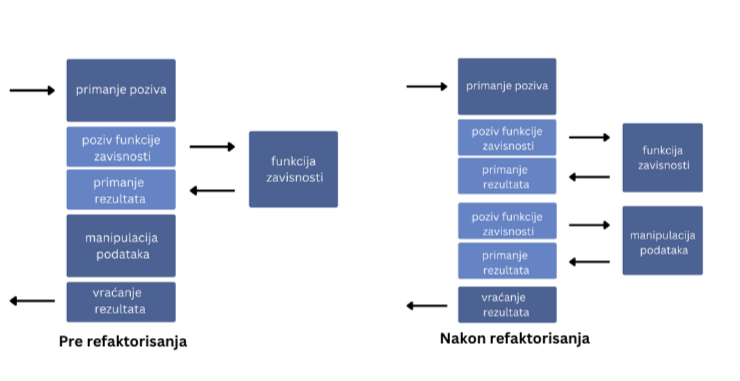
\includegraphics[width=0.9\textwidth]{dep.png}
  \caption{Izmeštanje koda u čistu funkciju}
\end{figure}

\par  U nekim slučajevima, nije lako odrediti šta se može izdvojiti u zasebnu funkciju. Tada postoji druga opcija za kreiranje kontrolisanog okruženja: napraviti zamenu za funkciju zavisnosti, i time izolovati k$\hat{o}$d. 

\subsection{Izolovanje koda} 
\par Ubrizgavanjem zavisnosti i kreiranjem dublera moguće je eliminisati spoljašnje promenljive, i time kontrolisati situaciju u kojoj k${o}$d koji se testira mora da se nađe. Tako se omogućava očekivanje nekog konkretnog rezultata. 
\par Zavisnost je bilo koji k$\hat{o}$d na koji se originalni k$\hat{o}$d oslanja. Korišćenjem DI (skraćenica za Dependency Injection) u testovima se kreiraju zamene zavisnosti koje se ponašaju na predvidljiv način, pa testovi mogu da se fokusiraju na logiku unutar koda koji se testira. U jediničnim testovima, najčešće se ubrizgava zavisnost tako što se prosledi kao parametar. Taj parametar može biti funkcija ili modul. Ubrizgavanje zavisnosti kroz API\footnote{skraćenica za aplikacioni veb interfejs (eng. \textit{web applicatoin
programming interface} )} obezbeđuje čist k$\hat{o}$d i jednostavne i kontrolisane jedinične testove. Sa druge strane, integracioni testovi zahtevaju drugačije metode ubrizgavanja zavisnosti. TODO nastavak...
\end{comment}



% The Elm compiler is quite capable of detecting many common errors. One of the major features of Elm that is frequently praised by developers, is its compiler error detection. Compiler error messages in Elm are user-friendly. These appear in the terminal or in the text editor if it is being used instead. They often contain suggestions or hints that are quite useful.
% https://medium.com/@cosc4315/elm-language-fine-tuning-e2dad1a33dad
% ------------------------------------------------------------------------------

\chapter{Portal MSNR}
\label{chp:msnr}

\par K$\hat{o}$d aplikacije pod nazivom \emph{Portal MSNR} koja će biti testirana javno je dostupan na \emph{GitHub-u} \cite{msnr-portal}. Portal MSNR je veb aplikacija namenjena praćenju i upravljanju aktivnostima kursa \emph{Metodologija stručnog i naučnog rada} \cite{rad}. Studenti na ovom kursu treba da steknu različite veštine koje se tiču pravilnog pisanja i recenziranja naučnih radova, pisanja CV-a, držanja prezentacija, i komunikacije u radu na timskim projektima. 

\section{Funkcionalnosti i osnovni entiteti portala}
\label{sec:entiteti}
\par Različite aktivnosti na kursu \emph{Metodologija stručnog i naučnog rada} implementirane su kao funkcionalnosti aplikacije. Korisnik portala može imati jednu od dve uloge: \emph{student} ili \emph{profesor}. Student na početku mora da podnese zahtev za registraciju, koju nakon toga odobrava profesor, i zatim student ima mogućnost da se prijavi na portal. Jedna od obaveza studenata na kursu jeste pisanje seminarskog rada --- profesor vrši odabir tema za tekuću godinu, a studenti treba da prijave svoju grupu za izradu seminarskog rada. Student ima i opciju da se prijavi za recenziranje radova drugih studenata, ukoliko to želi. Drugi zadatak koji se očekuje od studenata jeste pisanje CV-a. U okviru portala, student može priložiti tri različite vrste dokumenata --- prvu verziju seminarskog rada, recenzije, i svoju prvu verziju CV-a. Profesor, pored toga što vrši pregled zahteva za registraciju i odabir tema, ima mogućnost dodavanja svih aktivnosti tokom godine, i na kraju --- njihovo ocenjivanje.

\subsection{Entiteti}
\par Osnovni entiteti aplikacije predstavljeni su tabelama u bazi podataka i relacijama između njih.  Polazni entiteti su \emph{zahtev za registraciju studenata}, \emph{korisnik} i \emph{semestar}. U tabeli korisnika inicijalno postoji jedan nalog koji ima rolu profesora, a pri odobravanju registracije studenta kreira se nalog sa rolom studenta, i studentu se šalje elektronska pošta sa vezom za postavljanje lozinke. Pored unosa u tabelu \textit{users}, vrše se unosi u još dve tabele: \emph{students}, koja sadrži referencu ka korisniku i \emph{students{\textunderscore}semesters}, koja predstavlja relaciju između studenta i semestra, a ima i referencu ka tabeli \emph{groups} --- svaki student u toku jednog semestra može pripadati jednoj grupi. Nakon što profesor odabere teme za seminarske radove, vrši se unos u tabelu \emph{topics}, koja ima referencu ka semestru u kom se mogu odabrati. Prethodno navedeni tipovi aktivnosti predstavljeni su tabelom \emph{activity{\textunderscore}types}, a tabela \emph{activities} predstavlja relaciju između tipa aktivnosti i semestra. Tabela \emph{assignments} odnosi se na dodeljene aktivnosti koje mogu biti grupne ili individualne, te može imati referencu ka studentu ili ka grupi. Većina dodeljenih aktivnosti podrazumeva predaju dokumenata, koji će se nalaziti na serveru, a informacije o predatim dokumentima čuvaju se u tabeli \emph{documents}. Ova tabela sadrži referencu ka korisniku koji je priložio dokument, a tabela \emph{assignments{\textunderscore}documents} vezuje dokument i dodeljenu aktivnost.
\par Spisak naziva entiteta i tabela u okviru baze podataka koje njima odgovaraju dati su u tabeli \ref{tab:1}. Svaki od ovih entiteta, kao i relacije između njih, biće pojedinačno istestirani u narednom poglavlju.

\begin{table}[htb]
\centering
\caption{Entiteti portala i odgovarajuće tabele u bazi}
\label{tab:1}
\begin{tabular}{ |c|c| } 
 \hline
\textbf{Entitet} & \textbf{Tabele u bazi podataka} \\ 
 \hline
\textit{\textbf{Zahtev za registraciju studenata}} & \emph{student{\textunderscore}registrations}  \\ 
\textit{\textbf{Korisnik}} & \emph{users}  \\ 
\textit{\textbf{Semestar}} & \emph{semesters}  \\ 
\textit{\textbf{Student}} & \emph{students} i  \emph{student{\textunderscore}semester} \\ 
\textit{\textbf{Grupa}} & \emph{groups}  \\ 
\textit{\textbf{Tema seminarskog rada}} & \emph{topics}  \\
\textit{\textbf{Aktivnost}} & \emph{activities}  \\
\textit{\textbf{Tip aktivnosti}} & \emph{activity{\textunderscore}types} \\   
\textit{\textbf{Dodeljene aktivnosti}} & \emph{assignments}  \\
\textit{\textbf{Dokument}} & \emph{documents} i  \emph{assignments{\textunderscore}documents} \\
 \hline
\end{tabular}
\end{table}

\section{Arhitektura portala}
\label{sec:arhitektura}
\par Portal MSNR je primer klijent/server aplikacije koja se sastoji od tri sloja. Klijentski sloj implementiran je u programskom jeziku \emph{Elm}, kao jednostranična aplikacija (eng. \emph{Single Page Application --- SPA}) koja predstavlja korisnički interfejs. U sredini se nalazi aplikacioni veb interfejs koji je implementiran u programskom jeziku \emph{Elixir} pomoću razvojnog okvira \emph{Phoenix}, u stilu arhitekture \emph{REST} (eng. \emph{Representational State Transfer}) \cite{rest}. Treći sloj predstavlja relaciona baza podataka, i sistem za upravljanje bazom \emph{PostgreSQL} \cite{postgre}. Slika \ref{fig:msnr-arch} prikazuje navedenu arhitekturu. 

\begin{figure}[!ht]
  \centering
  \label{fig:msnr-arch}
  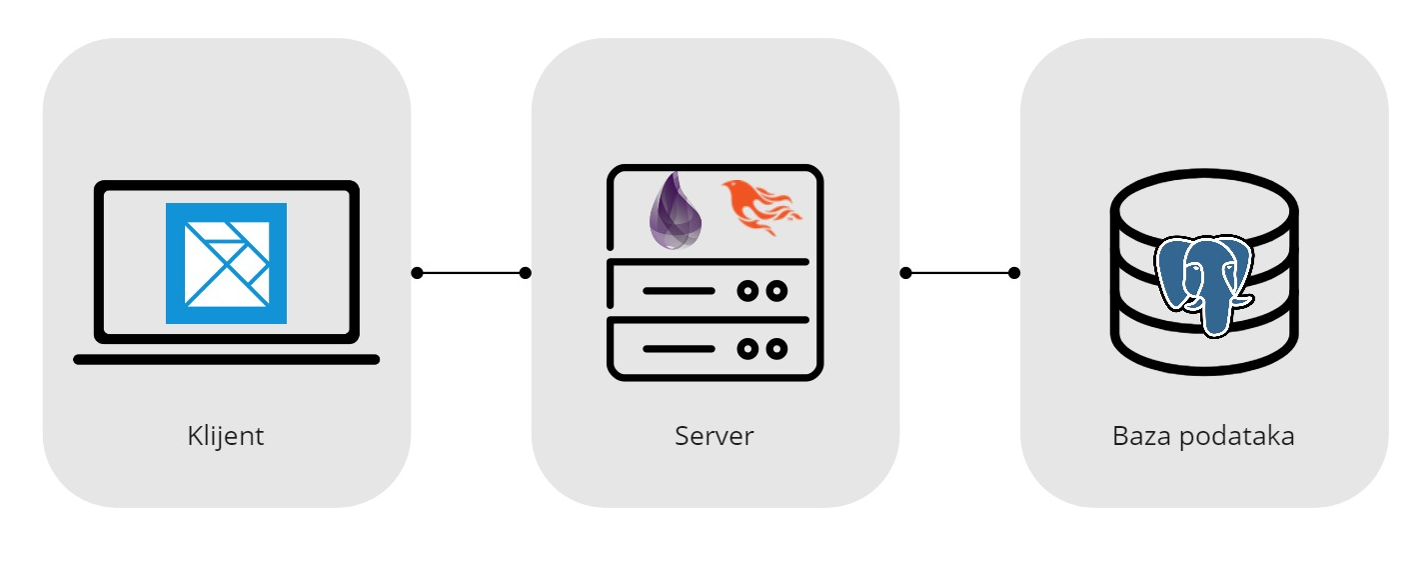
\includegraphics[width=0.9\textwidth]{msnr-arch.png}
  \caption{Arhitektura Portala MSNR \cite{rad}}
\end{figure}

\subsubsection{Struktura serverske strane portala}
\par U programskom jeziku Elixir, za razvoj veb aplikacija koristi se razvojni okvir \emph{Phoenix} \cite{phx}. Zasnovan je na obrascu \emph{model-pogled-upravljač} (eng. \emph{Model-View-Controller pattern, MVC}). Serverski deo aplikacija MSNR portal implementiran je kao \emph{Phoenix} projekat. Preciznije, projekat je u osnovi \emph{Mix} projekat, sa \emph{Phoenix} proširenjima. \emph{Mix} je osnovni alat ovog jezika koji se koristi za kreiranje, prevođenje i testiranje projekata. Pored ovog alata, potrebno je prethodno instalirati i menadžer paketa za ekosistem \emph{Erlang} pod nazivom \emph{Hex} \cite{hex}. Pri kreiranju \emph{Phoenix} projekta, dodeljeno mu je ime \emph{msnr{\textunderscore}api}. Na slici \ref{fig:msnr-str} je prikazana struktura projekta nakon uspešnog pokretanja komande za kreiranje. 

\begin{figure}[!ht]
  \centering
  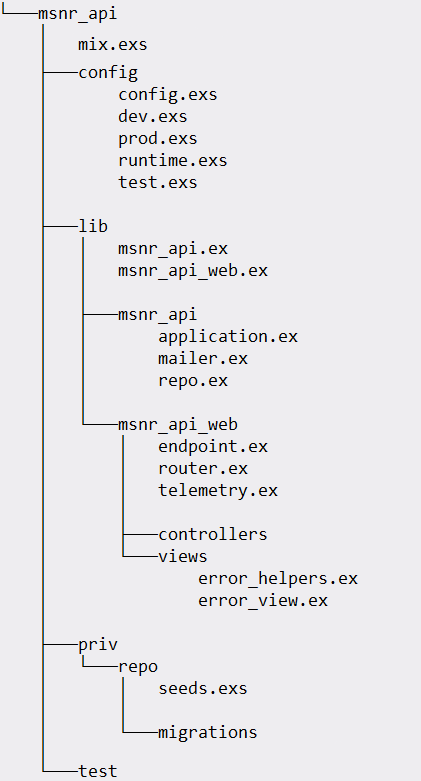
\includegraphics[width=0.5\textwidth]{msnr-str.png}
  \caption{Struktura \emph{Phoenix} projekta \emph{msnr{\textunderscore}api} \cite{rad}}
  \label{fig:msnr-str}
\end{figure}

\par U direktorijumu \emph{lib} nalaze se dva konteksta (eng. \emph{context}), tj. dva modula, od kojih svaki grupiše funkcije sa zajedničkom svrhom. Prvi kontekst je \emph{MsnrApi}, unutar koga je enkapsulirana sva domenska i poslovna logika, i definisani svi entiteti i funkcije za rad sa njima. Inicijalno su kreirana tri podmodula ovog konteksta: \emph{MsnrApi.Application}, koji pokreće aplikaciju, \emph{MsnrApi.Repo}, koji je zadužen za komunikaciju sa bazom, i \emph{MsnrApi.Mailer}, koji služi za slanje elektronske pošte. Drugi kontekst ima naziv \emph{MsnrApiWeb}, i on sadrži implementaciju za poglede i upravljače unutar arhitekture MVC. Njegovi podmoduli \emph{MnsrApiWeb.Endpoint} i \emph{MsnrApiWeb.Router} imaju ulogu u pripremi HTTP zahteva i njihovom prosleđivanju odgovarajućim upravljačima. 
\par Za sve obrade HTTP zahteva koristi se biblioteka \emph{Plug} \cite{plug}. Utikač (eng. \emph{plug}) je funkcija koja ima kao ulaznu i povratnu vrednost strukturu \emph{Plug.Conn} koja sadrži sve informacije o primljenom HTTP zahtevu. \emph{Phoenix} poziva utikače jedan za drugim, i svaki od njih transformiše ovu strukturu dok se obrada zahteva ne završi, i na kraju odgovor pošalje korisniku. Sa utikačima se povezuje veb server pod nazivom \emph{Cowboy}, a u mix.exs je automatski ubačena zavisnost \emph{plug{\textunderscore}cowboy}.
\par Kada se kreira novi \emph{mix} projekat, pored konfiguracione datoteke \emph{mix.exs}, i direktorijuma \emph{lib} koji sadrži osnovni k$\hat{o}$d aplikacije, kreira se i direktorijum \emph{test}. Unutar ovog direktorijuma će biti smešteni svi testovi vezani za serversku stranu aplikacije. 

\subsubsection{Struktura klijentske strane portala}
\par Klijent aplikacija Portala MSNR predstavlja jedan Elm projekat. U svakom Elm programu uočava se obrazac projektovanja koji se naziva \emph{Model-Pogled-Ažuriranje} (eng. \emph{Model View Update --- MVU}), ili \emph{Arhitektura Elm} \cite{elm-in-action}. Model predstavlja stanje aplikacije, pogled se odnosi na transformaciju stanja u HTML, a ažuriranje na promene stanja. Elm program radi tako što se generiše HTML koji se prikazuje u pretraživaču, a nakon toga pretraživač šalje poruku programu ako se nešto dogodi. Na osnovu primljene poruke funkcija \emph{update} kreira novi model, koji se prosleđuje funkciji \emph{view}, na osnovu koje se generiše HTML. Ovaj proces prikazan je na slici \ref{fig:elm-prog}. U arhitekturi Elm celokupno stanje aplikacije se nalazi na jednom mestu (u modelu), a protok podataka je uvek u jednom smeru.

\begin{figure}[!ht]
  \centering
  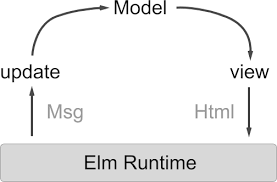
\includegraphics[width=0.4\textwidth]{elmprog.png}
  \caption{\emph{Arhitektura Elm} \cite{rad}}
  \label{fig:elm-prog}
\end{figure}


\par Inicijalizacija ovog projekta podrazumeva kreiranje jednog praznog direktorijuma \emph{src} i datoteke \emph{elm.json}, a sam korisnik odlučuje o organizaciji datoteka unutar projekta. Na slici \ref{fig:msnrelm} prikazano je rešenje organizacije Elm datoteka u okviru aplikacije Portal MSNR. 


\begin{figure}[!ht]
  \centering
  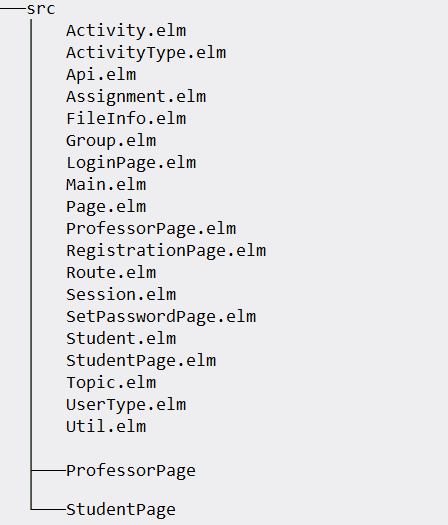
\includegraphics[width=0.6\textwidth]{msnr-elm.png}
  \caption{Struktura \emph{Elm} projekta \emph{msnr{\textunderscore}elm} \cite{rad}}
  \label{fig:msnrelm}
\end{figure}

\par U korenu projekta se nalazi osnovna datoteka \emph{Main.elm}, koja sadrži funkciju \emph{main} sa definicijom Elm aplikacije. Ostale datoteke sadrže definicije osnovnih stranica, entiteta, putanja i modula za komunikaciju sa serverom. U posebnim direktorijumima, izdvojene su datoteke za prikazivanje studentskih i profesorskih stranica. 
\par Korisnički interfejs portala implementiran je pomoću četiri funkcije: \emph{sandbox, element, document, application}. Ove funkcije se nalaze unutar modula \emph{Browser}, koji je deo paketa čija je uloga kreiranje Elm programa u pretraživaču. Funkcija \emph{sandbox} omogućava bazičnu interakciju sa korisnicima, bez komunikacije sa spoljnim svetom. Tu komunikaciju omogućava funkcija \emph{element}, pomoću koncepta komande, supskripcije, portova i oznaka (eng. \emph{flags}). Funkcija \emph{document} proširuje prethodnu funkciju tako što upravlja celim dokumentom i pruža kontrolu nad HTML elementima naslova i tela. Funkcija \emph{application} kreira aplikaciju koja upravlja url promenama. 
\par Aplikacija je kompajlirana tako da se kreira datoteka \emph{app.js}, koja se uključuje dokument \emph{index.html}. Pokreće se pozivanjem \emph{init} funkcije iz modula \emph{Main} i tada se vrši prosleđivanje putanje ka veb interfejsu preko oznaka. 
\par Elm aplikacija podeljena je na tri osnovna dela: stranice koje se koriste za prijavljivanje i registraciju korisnika, studentsku stranicu, i profesorske stranice. Pored njih, postoje i stranice koje nisu izdvojene u posebne module --- početna stranica i stranica koja se prikazuje u slučaju pogrešne putanje.


\section{Testiranje portala}
\par Testiranje ovakve aplikacije podrazumeva podelu na različite vrste testova. Za početak, jedinični testovi koji se odnose na individualne funkcije i upravljače koji barataju zahtevima u okviru serverskog dela aplikacije moraju biti napisani u programskom jeziku Elixir. Na serverskoj strani, potrebno je napisati i testove koji simuliraju zahteve API-ju i verifikuju odgovore od baze. Sa druge strane, jedinični testovi koji se fokusiraju na pojedinačne komponente i funkcije korisničkog interfejsa moraju biti napisani u programskom jeziku Elm. Nakon pojedinačnog testiranja klijentske i serverske aplikacije, slede integracioni testovi koji proveravaju kako korisnički interfejs funkcioniše zajedno sa API-jem. Na kraju je neophodno testirati celokupan sistem, od korisničkog interfejsa do baze podataka, pisanjem sistemskih testova. S obzirom na to da se radi o veb aplikaciji, mogu se sprovesti i testovi opterećenja koji će proveriti kako portal podnosi velike količine zahteva i korisnika. 
% TODO OVDE trbaju poporavke 
% U narednim poglavljima biće detaljno prikazano sprovođenje svih ovih testova.

\chapter{Testiranje serverskog dela aplikacije}
\label{chp:elixir}

\par U ovom poglavlju biće predstavljeni različiti koncepti testiranja u programskom jeziku \emph{Elixir}, kroz pisanje testova za serverski deo aplikacije Portal MSNR. \textit{ExUnit} je Elixir-ov ugrađeni razvojni okvir koji ima sve što je neophodno za iscrpno testiranje koda i biće osnova za sve testove kroz ovo poglavlje \cite{exunit}.

\section{Uvod u testiranje u okruženju ExUnit}
\label{sec:elixunit}

\par Pisanje testova u programskom jeziku \emph{Elixir} je moguće bez potrebe za drugim bibliotekama, jer je \emph{ExUnit} razvijan zajedno sa samim jezikom od početka. Svi testovi su implementirani kao \emph{Elixir} skripte, pa je pri davanju imena testu neophodno koristiti ekstenziju datoteke \emph{.exs}. Pre pokretanja testova potrebno je pokrenuti \emph{ExUnit}, kao što je prikazano u primeru koda \ref{lst:start}. Ova naredba se obično navodi unutar automatski generisane datoteke \emph{test/test{\textunderscore}helper.exs}. 

\begin{lstlisting}[language=elixir, caption={Pokretanje ExUnit},captionpos=b, label={lst:start}]
# test/test_helper.exs

ExUnit.start()
\end{lstlisting}

\par Testovi se pokreću najpre pozicioniranjem u direktorijum projekta, a zatim navođenjem komande \textbf{mix test}. Ova komanda pokreće sve testove koji se nalaze unutar \emph{test} direktorijuma. Navođenjem parametra \emph{--only} i imena testa ili modula može se pokrenuti specifičan test ili skup testova unutar jednog modula. Pozivanje naredbe \textbf{mix test } pokreće sve testove, i daje sledeći izlaz:  

\begin{lstlisting}[style=DOS]
PS C:\Users\panap\testing-msnr-portal\portal\msnr_api> mix test

..............
Finished in 0.2 seconds (0.00s async, 0.2s sync)
16 tests, 0 failures

Randomized with seed 801308
\end{lstlisting}

\par \emph{ExUnit} će testove izvršavati nasumičnim redosledom, koristeći ceo broj kao seme nasumičnosti (eng. \emph{randomization seed}). Poželjno je da se testovi izvršavaju slučajnim redosledom, jer se tako osigurava njihova izlovanost. Ako se desi da određeni test pada sporadično, to može biti jer neki od prethodnih testova menja stanje i ima posledice po druge testove. Ovako nešto može da se desi ako se testovi izvršavaju nekim određenim redosledom, i taj redosled se može dobiti pomoću ovog nasumičnog broja koji je dat u samom izlazu. Pokretanjem testova ponovo koristeći taj konkretni ceo broj kao seme nasumičnosti može se pronaći uzrok greške. 

\par Svita testova (eng. \emph{test suite}) je kolekcija testova slučajeva upotrebe, koji imaju isti posao, ali različite scenarije. Ona može služiti kao dokumentacija, sa opisima o očekivanom ponašanju koda, tako da treba voditi računa da bude dobro organizovana. \emph{ExUnit} dolazi sa veoma korisnim funkcijima i makroima koji omogućavaju tu organizaciju u jednu čitljivu i održivu datoteku. Alat \emph{describe} omogućava davanje opisa grupe testova, kao i dodeljivanja zajedničke pripreme podataka za celu grupu. Preporuka je za početak grupisati testove po funkciji, kao što je prikazano u primeru koda \ref{lst:desc}, ali odluka o načinu grupisanja je na pojedincu. Svrha je čitljivost i lakše razumevanje.
\par Testovi u \emph{Elixir} projektima se organizuju u module i test slučajeve. U ovom primeru, modul pod nazivom \emph{MsnrApi.UnitTests.PasswordTest} sadrži jedinične testove koji se odnose na kontekst koji opisuje šifre korisnika (\emph{MsnrApi.Accounts.Password}). Blok \emph{describe} se sastoji od dva test slučaja i odnosi se na funkcije hash i \emph{verify{\textunderscore}with{\textunderscore}hash}. Njihova uloga je da hešuju lozinku upotrebom nasumične tzv. \emph{salt} niske i zatim verifikuju da je lozinka ispravno heširana, tj. zaštićena tako da postoji kao nasumična niska u bazi. Više o ovim funkcijama može se naći u dokumentaciji Eliksirovog modula \emph{Pbkdf2} \cite{pbk}. Navođenjem ključne reči test, a za njom niske koja treba da opiše šta je to što test treba da uradi, definiše se jedna funkcija koja predstavlja test slučaj. U primeru koda \ref{lst:desc} data su dva test slučaja, od kojih jedan proverava uspešno izvršavanje funkcije kada se prosledi ispravna lozinka funkciji \emph{verify{\textunderscore}with{\textunderscore}hash}, a drugi proverava da li se javlja greška kada se prosledi neodgovarajuća niska. 
 
% \par Testovi u Elixir projektima se organizuju u module i test slučajeve. U ovom primeru, modul pod nazivom \emph{AccountsTest} sadrži testove koji se odnose na kontekst koji opisuje korisnike. Blok \emph{describe} iz primera se sastoji od dva test slučaja, i odnosi se na funkciju \emph{get{\textunderscore}user}, koja vrši jednostavno dohvatanje korisnika iz baze prosleđivanjem identifikatora. Navođenjem ključne reči \emph{test}, a za njom niske koja treba da opiše šta je to što test treba da uradi, definiše se jedna funkcija koja predstavlja test slučaj. Na primeru \emph{describe} bloka funkcije \emph{get{\textunderscore}user}, prikazana su dva test slučaja, od kojih jedan proverava uspešno izvršavanje funkcije kada se prosledi validan identifikator, a drugi proverava da li se javlja greška kada se prosledi identifikator korisnika koji ne postoji. Deo koda koji se odnosi na samo ubacivanje korisnika u bazu podataka, upotreba koncepta fabrike, kao i vraćanje baze na prvobitno stanje biće detaljno objašnjeni u delu \ref{sec:baza}.
\par Unutar jednog test slučaja poziva se funkcija ili upravljač i proverava se očekivani rezultat. Makroom \emph{assert} se testira da li je izraz istinit. U slučaju da nije, test ne prolazi i izbacuje grešku. Ako funkcija \emph{verify{\textunderscore}with{\textunderscore}hash} vrati \emph{true}, ovaj test uspešno prolazi. Na primeru testa koji proverava neuspešnu putanju izvršavanja, koristi se makro \emph{refute}, koji se koristi kada je potrebno proveriti da li je izraz neistinit (eng. \emph{false}) . U ovom slučaju očekuje se da funkcija vrati false kada joj se prosledi neispravna lozinka.



\begin{lstlisting}[language=elixir, caption={Opisivanje testova unutar jedne grupe, na primeru funkcije za verifikaciju lozinke},captionpos=b, label={lst:desc}]
defmodule MsnrApi.UnitTests.PasswordTest do
...
  describe "verify password" do
    test "success: verifies the password by hashing" do
      password = "somepass123"

      assert hash = Password.hash(password)
      assert Password.verify_with_hash(password, hash) == true
    end

    test "error: returns false when given wrong password" do
      password = "somepass123"
      wrong = "wrong"

      assert hash = Password.hash(password)
      refute Password.verify_with_hash(wrong, hash)
    end
  end
\end{lstlisting}


\par U slučaju da leva i desna strana izraza navedenog nakon makroa \emph{assert} nisu jednake, test ne prolazi, a \emph{ExUnit} daje obaveštenje o tome koji od testova su neuspešni, kao i koje su prava i očekivana vrednost. Izlaz koji se dobije u slučaju da rezultat izvršavanja funkcije nije onaj koji je očekivan, prikazan je na listingu \ref{lst:term}. 

\begin{lstlisting}[style=DOS, caption={Izlaz u slučaju testa koji ne prolazi},captionpos=b, label={lst:term}]
1) test verify password success: verifies the password by hashing (MsnrApi.UnitTests.PasswordTest)
   test/msnr_api/unit_tests/password_test.exs:6
   Assertion with == failed
   code:  assert Password.verify_with_hash(password, hash) == true
   left:  false
   right: true
   stacktrace:
     test/msnr_api/unit_tests/password_test.exs:10: (test)
.
Finished in 5.0 seconds (0.00s async, 5.0s sync)
2 tests, 1 failure

\end{lstlisting}


\par Pored najčešće korišćenog makroa \emph{assert}, \emph{ExUnit} nudi još nekoliko njih koji se mogu koristiti u različitim situacijama. U narednoj listi dati su nazivi i opisi nekih takvih makroa:
 \begin{itemize}
 \item \emph{assert{\textunderscore}raise} --- koristi se kada je potrebno utvrditi da je podignut odgovarajući izuzetak. 
 \item \emph{assert{\textunderscore}receive} --- koristi se kada je potrebno proveriti da li je proces primio konkretnu poruku.
 \item \emph {capture{\textunderscore}io} --- koristi se kada je potrebno proveriti da li se na standardanom izlazu ispisuje očekivano.
 \item \emph{capture{\textunderscore}log} --- koristi se kada je potrebno proveriti sadržaj log poruka, npr. pri pozivu \emph{Logger.info}.
 \item \emph{setup i setup{\textunderscore}all} --- koriste se kada je potrebno izvršiti pripremu testova, pokreću se pre svakog testa, ili pre jedne grupe.
 \end{itemize}
 
\par Upotreba makroa \emph{setup} i \emph{assert{\textunderscore}raise} prikazana je u primeru dela koda \ref{lst:del}. K$\hat{o}$d  unutar makroa \emph{setup} će se pokretati pre svakog testa, a u ovom primeru priprema podrazumeva eksplicitno dohvatanje konekcije sa bazom podataka pre izvršavanja svakog od testova. Povezivanje sa bazom podataka biće detaljno objašnjeno u narednoj sekciji. Test slučaj iz ovog primera pokriva neuspešan slučaj funkcije \emph{get{\textunderscore}user} koja treba da dohvati korisnika iz baze. Pri pokušaju dohvatanja nepostojećeg korisnika, očekuje se izuzetak tipa \emph{NoResultsError}.
 
\begin{lstlisting}[language=elixir, caption={Upotreba makroa \emph{setup} i \emph{assert{\textunderscore}raise} na primeru funkcije \emph{get{\textunderscore}user}},captionpos=b, label={lst:del}]
setup do
    Ecto.Adapters.SQL.Sandbox.checkout(MsnrApi.Repo)
end
  
describe "get_user/1" do
...
    test "error: it returns an Ecto.NoResultsError when a user doesn't exist" do

      invalid_id = -1
      assert_raise Ecto.NoResultsError, fn ->
        Accounts.get_user!(invalid_id) end
    end
  end
\end{lstlisting}


\section{Testiranje komunikacije sa bazom podataka}
\label{sec:baza}

\par Kod testiranja spoljašnjih entiteta i servisa koji su van kontrole pojedinca koji piše ili testira kod, često se koristi proces koji se naziva mokovanje (eng. \emph{mocking}) \cite{external}. Mokovanje podrazumeva simuliranje tih spoljašnjih entiteta, bez njihove stvarne upotrebe. Glavna svrha ovog procesa jeste izolacija jedinice koja se testira, bez uticaja ponašanja eksternih entiteta. Primer jednog takvog entiteta je baza podataka. Umesto prave baze, mogu se koristiti kontrolisani objekti koji će simulirati njeno ponašanje. Jedinični testovi tako mogu da pokriju neke kompleksne manipulacije sa podacima iz baze, a da se pritom ne koristi pravi sadržaj baze koji u tom trenutku nije važan. 
\par U kontekstu ovog projekta, baza podataka je sastavni deo aplikacije i nad njom postoji potpuna kontrola. Ona se može pokretati i zaustavljati po želji, i nema nepredviđenih rizika u njenom ponašanju. Takođe, operacije koje su testirane u ovom delu su jednostavni upiti i načini interakcije sa bazom. S obzirom na to da ne postoji dodatna logika koju je potrebno testirati u izolaciji, u ovoj situaciji nije primenljivo mokovanje. Svi testovi unutar kojih se komunicira sa bazom podataka će ostvarivati prave konekcije i dohvatati stvarne podatke iz baze. Ovakvi testovi blisko oslikavaju kako bi se aplikacija ponašala i u produkciji. Dodatno vreme izvršavanja koje zahteva pristupanje bazi je u ovom slučaju prihvatljivo.

\subsection{Testiranje u okruženju Ecto}
\par Biblioteka \emph{Ecto} zadužena je za sve interakcije sa relacionim bazama podataka u \emph{Elixir} okruženju \cite{ecto}. Pored komunikacije sa bazom, \emph{Ecto} ima i ulogu u validaciji. Moduli ove biblioteke koje je značajno naglasiti su: \emph{Ecto.Repo}, \emph{Ecto.Schema} i \emph{Ecto.Changeset}. \emph{Ecto.Repo} opisuje gde se nalaze podaci, odnosno definiše omotač oko baze preko kog se ostvaraje komunikacija sa bazom. \emph{Ecto.Schema} ima ulogu u definisanju mapiranja eksternih podataka u \emph{Elixir} strukture. Koncept skupa promena (eng. \emph{changeset}) odnosi se na proces validacije podataka, njihovog konvertovanja i provere dodatnih uslova pre nego što se upišu u bazu. \emph{Ecto.Changeset} modul opisuje kako se menjaju podaci. U ovom delu, prikazani su testovi koji proveravaju da li k$\hat{o}$d koristi funkcionalnosti biblioteke \emph{Ecto} na ispravan način.
\par \emph{Ecto} i svi potrebni moduli se podrazumevano uključuju prilikom kreiranja \emph{Phoenix} projekta. Pre samog pisanja testova, neophodno je podesiti sve parametre za komunikaciju sa bazom podataka \emph{PostgreSQL} u testnom okruženju. U datoteci \emph{config/test.exs} potrebno je uneti podatke kao što je prikazano u primeru koda \ref{lst:conf}. Pokretanjem naredbe \emph{MIX{\textunderscore}ENV=test mix ecto.create} iz komandne linije, lokalno će se kreirati \emph{msnr{\textunderscore}api{\textunderscore}test} baza podataka.

\begin{lstlisting}[language=elixir, caption={Konfiguracija baze podataka u testnom okruženju},captionpos=b, label={lst:conf}]
  config :msnr_api, MsnrApi.Repo,
  username: "postgres",
  password: "1234",
  database: "msnr_api_test#{System.get_env("MIX_TEST_PARTITION")}",
  hostname: "localhost",
  pool: Ecto.Adapters.SQL.Sandbox,
  pool_size: 10
\end{lstlisting}

\par Svi testovi u ovom delu nalaze se u direktorijumima \textit{'/test/msnr{\textunderscore}api/schema'} i \textit{'/test/msnr{\textunderscore}api/queries'}, u okviru projekta \emph{msnr{\textunderscore}api}. 
\par Na početku, napisani su jednostavni testovi koji proveravaju ispravnost definisanja struktura pomoću \emph{Ecto.Schema} modula. Primer definisanja entiteta dodeljenih aktivnosti  dat je u primeru koda \ref{lst:schema}. Pomoću makroa \emph{schema} i \emph{field} definišu se tabele, njihova polja i relacije sa drugim tabelama. Oni istovremeno definišu i Elixir strukturu --- u ovom primeru, ta struktura se naziva \emph{Assignment}. Pored ovog, i svi ostali entiteti su definisani kao konteksti u okviru konteksta \emph{MsnrApi}, koji sadrži domensku logiku aplikacije. Funkcija \emph{changeset/2} biće objašnjena u delu koji govori o testiranju skupa promena.

\begin{lstlisting}[language=elixir, caption={Shema tabele \emph{assignments}},captionpos=b, label={lst:schema}]
defmodule MsnrApi.Assignments.Assignment do
  use Ecto.Schema
  import Ecto.Changeset

  schema "assignments" do
    field :comment, :string
    field :completed, :boolean, default: false
    field :grade, :integer
    field :student_id, :id
    field :group_id, :id
    field :activity_id, :id
    field :related_topic_id, :id
    timestamps()
  end

  def changeset(assignment, attrs) do
    assignment
    |> cast(attrs, [:comment, :grade])
    |> validate_required([:comment, :grade])
  end
...
\end{lstlisting}

\subsection{Testiranje polja i tipova}
\par Test koji proverava polja i tipove tabele \emph{assignments} dat je u kodu \ref{lst:testschema}. Ovo je primer jednostavnog testa koji proverava da li definisana shema ima tačna polja i odgovarajuće tipove. Unutar testa se prvo prolaskom kroz sva polja strukture \emph{Assignment} izvuku polje i njegov tip, i zatim se navodi ključna reč \emph{assert}, kojom se proverava da li su prava polja i tipovi jednaki očekivanim. Lista \emph{@expected{\textunderscore}fields{\textunderscore}with{\textunderscore}types} definisana je kao lista parova polja i odgovarajućih tipova, kao što su navedeni u primeru \ref{lst:schema}. Unutar \emph{assert} naredbe, i prava i očekivana lista pretvorene su u \emph{MapSet} strukturu, kako bi se redosledi polja poklapali sa obe strane. Slični testovi napisani su i za sve ostale entitete navedene u sekciji \ref{sec:entiteti}.

\begin{lstlisting}[language=elixir, caption={Test za proveru polja i tipova tabele \emph{assignments}},captionpos=b, label={lst:testschema}]
defmodule MsnrApi.Schema.AssignmentTest do
...  
  describe "fields and types" do
    test "it has the correct fields and types" do
      actual_fields_with_types =
        for field <- Assignment.__schema__(:fields) do
          type = Assignment.__schema__(:type, field)
          {field, type}
         end
    
      assert MapSet.new(actual_fields_with_types) == MapSet.new(@expected_fields_with_types)
  end
 end
\end{lstlisting}

\subsection{Testiranje skupa promena}
\label{sec:change}
\par Funkcija \emph{changeset} iz primera koda \ref{lst:schema} obuhvata različite transformacije podataka, kao i njihovu validaciju pre unosa u bazu podataka. Svrha ove funkcije je da svi podaci koji se unose ili ažuriraju u bazi budu ispravni i u skladu sa zahtevima aplikacije. Svaka od shema ima svoju definiciju polja i svoju \emph{changeset} funkciju. Tokom razvoja aplikacije, shemama se mogu dodavati različite izmene, kao što su nova polja, ili izmene u samim validacijama unutar funkcije \emph{changeset}. Funkcija \emph{cast} je prva u nizu funkcija koje se pozivaju i ona ograničava polja koja se mogu menjati. U slučaju modula \emph{Assignment}, to su polja \emph{comment} i \emph{grade}. Funkcija \emph{validate{\textunderscore}required} proverava obavezna polja. Rezultat izvršavanja ovih funkcija je takođe \emph{Ecto.Changeset} struktura, koja sadrži informacije o promenama koje treba izvršiti, validnost izmena i greške validacije ukoliko one postoje.
\par Testovi koji se odnose na ove funkcije implementirani su unutar \emph{describe} bloka \emph{''changeset/2''}, za svaki od entiteta aplikacije. Oni pokrivaju i uspešan scenario, i neke od slučajeva greški. Koji od ovih scenarija će se desiti, zavisi od ispravnosti prosleđenih parametara funkcije. Parametri koji će se prosleđivati u testovima formirani su unutar pomoćnih funkcija koje se nalaze u modulu \emph{SchemaCase}. On se nalazi u direktorijumu \emph{msnr{\textunderscore}api/test/support}, zajedno sa ostalim datotekama koje sadrže zajednički k$\hat{o}$d. Da bi ova datoteka bila prepoznata kada se pokreću testovi, potrebno je dodati dve linije unutar \emph{mix.exs} datoteke, koje su prikazane u kodu \ref{lst:mst}. Ovime se govori aplikaciji da uključi sve datoteke u \emph{test} direktorijumu prilikom kompilacije u testnom okruženju. Tako \emph{SchemaCase} postaje dostupan isključivo prilikom testiranja.

\begin{lstlisting}[language=elixir, caption={Uključivanje datoteka iz test direktorijuma pri kompilaciji u testnom okruženju},captionpos=b, label={lst:mst}]
defp elixirc_paths(:test), do: [''lib'', ''test'']
defp elixirc_paths(_), do :[''lib'']
...
def project do [
     ...
     elixirc_paths: elixirc_paths(Mix.env()), 
]
\end{lstlisting}

\par Što se tiče faze rušenja, \emph{Ecto} obezbeđuje da svaki pojedinačni test ne mora da prati okruženje i vraća ga na prvobitno stanje. Za to je zadužen \emph{Ecto.Sandbox}, koji omogućava paralelno izvršavanje testova bez deljenog stanja u bazi podataka i automatski vrši poništavanje svih promena u bazi na kraju svakog testa. Konfiguracija je prikazana u primeru koda \ref{lst:sand}. U datoteci \emph{schema{\textunderscore}case} potrebno je dodati \emph{setup} blok koji će svi testovi koji koriste ovaj obrazac pokretati na početku izvršavanja. Manuelni režim podrazumeva da će svaki test moći da zahteva svoju \emph{Sandbox} konekciju. Takođe, u konfiguracionoj datoteci \emph{config/test.exs}, u \emph{Ecto} delu, dodaju se linije koje obaveštavaju \emph{Ecto} da će se koristiti \emph{Sandbox}. Ovime se obezbeđuje da nijedan test u kome su vršene izmene u samoj bazi ne mora da ima eksplicitnu fazu rušenja --- na kraju testa baza se automatski vraća u prvobitno stanje. 
%TODO sta je connection pool?? kako prevesti
\begin{lstlisting}[language=elixir, caption={Podešavanje \emph{Ecto.Sandbox}},captionpos=b, label={lst:sand}]

# msnr_api/test/schema_case.ex
setup do
    Ecto.Adapters.SQL.Sandbox.mode(MsnrApi.Repo, :manual)
end
...
# msnr_api/config/test.exs
config :msnr_api, MsnrApi.Repo,
  database: "msnr_api_test",
  pool: Ecto.Adapters.SQL.Sandbox,
\end{lstlisting}

\subsubsection{Generisanje lažnih podataka}
\par Za potrebe testiranja svih entiteta, biće neophodno obezbediti lažne podatke odgovarajućih tipova koji će odgovarati poljima u tabelama. Modul \emph{SchemaCase} je jedan od pomoćnih modula u kojem se nalaze funkcije koje će se pozivati u skoro svim testovima koji proveravaju sheme u okviru baze podataka. Sadrži dve funkcije, od kojih jedna konstruiše realistične podatke ispravnih tipova, a druga konstruiše podatke koji su pogrešnog tipa u odnosu na polje tabele. 
\par Za generisanje nasumičnih realističnih podataka korišćena je biblioteka \emph{Faker} \cite{faker}. \emph{Faker} je potrebno uključiti u zavisnosti projekta, dodavanjem linije \textit{\{:faker, ''$\sim$> 0.17'', only: :test\}} u \emph{deps} delu konfiguracione datoteke \emph{mix.exs}. Biblioteku nije potrebno koristiti u razvojnom i produkcionom okruženju, te se ovom linijom ograničava njena upotreba samo na testno okruženje. U tabeli \ref{tab:fake} prikazani su neki od modula biblioteke \emph{Faker} i njhove funkcije koje su korišćene prilikom generisanja podataka za testiranje.

\begin{table}[!htbp]
\centering
\caption{Moduli biblioteke \emph{Faker}}
\label{tab:fake}
\begin{center}
\begin{tabular}{ | m{3cm} | m{5cm}| m{10em} | } 
 \hline
\textbf{Modul} & \textbf{Funkcije modula} & \textbf{Opis funkcija} \\ 
  \hline
 \textit{\textbf{Faker.Lorem}} &\emph{\small{characters() \newline paragraph() \newline sentence() \newline word()}} & \small{generisanje nasumičnih karaktera, paragrafa, rečenica ili pojedinačnih reči} \\ 
  \hline
 \textit{\textbf{Faker.Person}} &\emph{\small{first{\textunderscore}name() \newline last{\textunderscore}name() \newline title()}} & \small{generisanje nasumičnih podataka u vezi sa osobom --- ime, prezime, ili zvanje} \\ 
  \hline
 \textit{\textbf{Faker.Internet}} &\emph{\small{email() \newline url() \newline domain{\textunderscore}name()}} & \small{generisanje nasumičnih podataka sa Interneta --- imejl adrese, url putanje, nazivi domena} \\ 
 \hline
 \textit{\textbf{Faker.Random}} &\emph{\small{random{\textunderscore}between(int, int) \newline random{\textunderscore}uniform()}} & \small{generisanje nasumičnih celih i realnih brojeva} \\ 
\hline
\textit{\textbf{Faker.File}} &\emph{\small{file{\textunderscore}extension() \newline file{\textunderscore}name()}} & \small{generisanje nasumičnih ekstenzija i imena datoteka} \\ 
\hline
\textit{\textbf{Faker.Date}} &\emph{\small{backward(days) \newline forward(days)}} & \small{generisanje nasumičnih datuma određeni broj dana unazad ili unapred} \\ 
\hline

\end{tabular}
\end{center}
\end{table}


\par Pomoćne funkcije \emph{valid{\textunderscore}params} i \emph{invalid{\textunderscore}params} iz modula \emph{SchemaCase} prikazane su u primeru koda \ref{lst:faker}. Ove funkcije kao povratnu vrednost imaju mapu koja sadrži niske naziva polja kao ključeve, i odgovarajuće generisane vrednosti koje njima odgovaraju. Prva funkcija generiše realistične podatke ispravnog tipa, i ona se poziva u testovima koji proveravaju ispravnu putanju. Druga funkcija generiše podatke neodgovarajućeg tipa i ona u testovima služi za sprovođenje neuspešne putanje izvršavanja. Na primer, za polja koja bi trebalo da budu niske, ova funkcija generiše podatak tipa \emph{DateTime}.

\begin{lstlisting}[language=elixir, caption={Definicije pomoćnih funkcija \emph{valid{\textunderscore}params} i \emph{invalid{\textunderscore}params}},captionpos=b, label={lst:faker}]

def valid_params(fields_with_types) do

    valid_value_by_type = %{
      string: fn -> Faker.Lorem.word() end,
      naive_datetime: fn -> Faker.Date.backward(Enum.random(0..100)) end,
      id: fn -> Enum.random(0..100) end,
      ... 
    }

    for {field, type} <- fields_with_types, into: %{} do
      case field do
        {Atom.to_string(field), valid_value_by_type[type].()}
      end
    end
  end

  def invalid_params(fields_with_types) do
    invalid_value_by_type = %{
      string: fn -> DateTime.utc_now() end,
      naive_datetime: fn -> Faker.Lorem.word() end,
      id: fn -> DateTime.utc_now() end,
      ...
    }

    for {field, type} <- fields_with_types, into: %{} do
      {Atom.to_string(field), invalid_value_by_type[type].()}
    end
  end

\end{lstlisting}

\subsubsection{Testiranje funkcija changeset}

\par Funkcija \emph{changeset/2} iz primera koda \ref{lst:schema}, koja kao argumente prihvata strukturu \emph{Assignment} i listu atributa, ima ulogu da validira prisustvo dva polja u tabeli \emph{assignments} --- polja \emph{comment} i \emph{grade}. Test slučaj koji proverava uspešnu putanju izvršavanja funkcije \emph{changeset/2} prikazan je u primeru koda \ref{lst:changeset}. Funkciji se prosleđuju validni parametri, kreirani pomoću prethodno definisane funkcije \emph{valid{\textunderscore}params}. Nakon toga, proverava se da li je dobijeni skup promena validan, a onda se pojedinačno za svako neophodno polje proverava da li je ispravno.

\begin{lstlisting}[language=elixir, caption={Test slučaj uspešne upotrebe funkcije \emph{changeset/2}},captionpos=b, label={lst:changeset}]
  test "success: returns a valid changeset when given valid arguments" do
      valid_params = valid_params(@required_fields)
      changeset = Assignment.changeset(%Assignment{}, valid_params)

      assert %Changeset{valid?: true, changes: changes} = changeset

      for {field, _} <- @required_fields do
        actual = Map.get(changes, field)
        expected = valid_params[Atom.to_string(field)]
        assert actual == expected,
          "Values did not match for: #{field}\nexpected: #{inspect(expected)}\nactual: #{inspect(actual)}"
      end
  end 
\end{lstlisting}

\par Drugi test slučaj koji je potrebno pokriti je slučaj kada dolazi do greške zbog prosleđenih parametara koji nisu ispravni. Funkciji \emph{changeset} se proslede parametri formirani pomoću funkcije \emph{invalid{\textunderscore}params}, i očekuje se da će dobijeni skup promena biti nevalidan. Nakon te provere, proverava se lista grešaka, koja bi trebalo da sadrži svako od neophodnih polja. Pošto su prosleđeni parametri pogrešnog tipa, koji se ne može kastovati u odgovarajući ispravni tip, očekuje se da u okviru greške, vrsta validacije bude \emph{:cast}, pa se i to na kraju proverava još jednom \emph{assert} naredbom. Ovaj test slučaj prikazan je u primeru koda \ref{lst:cast}. 

\begin{lstlisting}[language=elixir, caption={Test slučaj neuspešne upotrebe funkcije \emph{changeset/2}, prosleđivanjem neodgovarajućih parametara},captionpos=b, label={lst:cast}]
test "error: returns an invalid changeset when given uncastable values" do
      invalid_params = invalid_params(@required_fields)

      assert %Changeset{valid?: false, errors: errors} = Assignment.changeset(%Assignment{}, invalid_params)

      for {field, _} <- @required_fields do
        assert errors[field], "the field: #{field} is missing from errors."

        {_, meta} = errors[field]
        assert meta[:validation] == :cast,
          "The validation type #{meta[:validation]} is incorrect."
      end
end
\end{lstlisting}

\par Ako se funkciji \emph{changeset} prosledi prazna mapa, tj. ako nedostaju polja koja inače moraju biti navedena, javlja se greška čiji je tip validacije \emph{:required}. Primer ovog test slučaja dat je u kodu \ref{lst:req}. U ovom slučaju, nakon provere da li je skup promena neispravan, proverava se da li je svako od zahtevanih polja u listi grešaka, a nakon toga i da li je tip validacije \emph{:required}. Na kraju, pomoću \emph{refute} naredbe, utvrđuje se da se opciona polja ne nalaze u listi grešaka. To su polja koja nije neophodno navesti pri pozivanju ove funkcije, i oni se zato ne trebaju naći ni među greškama.

\begin{lstlisting}[language=elixir, caption={Test slučaj neuspešne upotrebe funkcije \emph{changeset/2}, sa nedostajućim parametrima},captionpos=b, label={lst:req}]
test "error: returns an error changeset when required fields are missing" do
      params = %{}
      assert %Changeset{valid?: false, errors: errors} = Assignment.changeset(%Assignment{}, params)

      for {field, _} <- @required_fields do
        assert errors[field], "The field #{field} is missing from errors."
        {_, meta} = errors[field]
        assert meta[:validation] == :required,
        "The validation type #{meta[:validation]} is incorrect."
      end

      for field <- @optional_fields do
        refute errors[field], "The optional field #{field} is required when it shouldn't be."
      end
end
\end{lstlisting}

\par Neke od shema će unutar svoje \emph{changeset} funkcije imati i dodatne validacije, kao što je na primer validacija jedinstvenih polja. Na primeru sheme \emph{users}, nakon ostalih izmena i validacija, dodat je i sledeći poziv funkcije: \emph{unique{\textunderscore}constraint(:email)}. Ova funkcija obaveštava \emph{Ecto} da u tabeli korisnika ne sme postojati dva korisnika sa istom imejl adresom, tj. polje \emph{:email} mora biti jedinstveno za svakog korisnika. Ako se desi pokušaj registrovanja korisnika sa već iskorišćenom imejl adresom, dolazi do greške tipa \emph{:unique}. Ovaj test slučaj prikazan je u primeru koda \ref{lst:uniq}. Neophodno je ostvariti direktan pristup bazi podataka, pa je prva linija unutar test slučaja naredba kojom se kreira konekcija sa bazom. Zatim se u bazu ubacuje novi korisnik (pozivom \emph{MsnrApi.Repo.insert()}), i time je završena priprema testa. Nakon toga, pokušava se ubacivanje još jednog korisnika sa istom imejl adresom. To bi trebalo da izazove grešku, što se proverava prvom naredbom \emph{assert}. Druga naredba \emph{assert} proverava da li se greška odnosi na polje \emph{:email}, a treća utvrđuje i tačnu vrstu greške, slično kao u prethodnim primerima. Za razliku od prethodnih testova, meta podaci u ovom slučaju nisu validacija, već ograničenje (eng. \emph{constraint}). 

\begin{lstlisting}[language=elixir, caption={Test slučaj neuspešne upotrebe funkcije \emph{changeset/2}, pri narušavanju ograničenja jedinstvenosti},captionpos=b, label={lst:uniq}]
test "error: returns an error changeset when an email is reused" do
      Ecto.Adapters.SQL.Sandbox.checkout(MsnrApi.Repo)

      {:ok, existing_user} =
        %User{}
        |> User.changeset(valid_params(@required_fields))
        |> MsnrApi.Repo.insert()
        
      changeset_with_reused_email =
        %User{}
        |> User.changeset(valid_params(@required_fields)
        |> Map.put("email", existing_user.email))

      assert {:error, %Changeset{valid?: false, errors: errors}} =
        MsnrApi.Repo.insert(changeset_with_reused_email)

      assert errors[:email], "The field :email is missing from errors."
      {_, meta} = errors[:email]

      assert meta[:constraint] == :unique,
      "The validation type #{meta[:validation]} is incorrect."
    end
\end{lstlisting}

\subsection{Testiranje upita}
\par U ovom delu biće prikazano kako su testirani konteksti entiteta. Modul koji će služiti kao primer se odnosi na korisnike --- \emph{MsnrApi.Accounts}. Struktura jednog dela ove datoteke prikazana je u primeru koda \ref{lst:act}, gde se može videti upotreba funkcija za interakciju sa bazom podataka kroz modul \emph{Ecto.Repo}. Prikazane su osnovne operacije dohvatanja redova iz tabele, dodavanja novog reda, ažuriranja reda, i brisanja reda iz zadate tabele. Unutar funkcija \emph{create{\textunderscore}user} i \emph{update{\textunderscore}user} poziva se i funkcija \emph{User.changeset}, koja je već prethodno istestirana.  

\begin{lstlisting}[language=elixir, caption={Definicija modula \emph{MsnrApi.Accounts}},captionpos=b, label={lst:act}]
defmodule MsnrApi.Accounts do
  alias MsnrApi.Repo
  alias MsnrApi.Accounts.User

 def list_users do
    Repo.all(User)
  end
  
  def get_user!(id), do: Repo.get!(User, id)

  def create_user(attrs \\ %{}) do
    %User{}
    |> User.changeset(attrs)
    |> Repo.insert()
  end

  def update_user(%User{} = user, attrs) do
    user
    |> User.changeset(attrs)
    |> Repo.update()
  end

  def delete_user(%User{} = user) do
    Repo.delete(user)
  end
\end{lstlisting}

\subsubsection{Fabrike za pripremu podataka}
\par Prilikom pisanja testova koji pristupaju tabelama baze podataka, za dohvatanje podataka u fazi pripreme, pogodno je iskoristiti obrazac fabrike (eng. \emph{factory pattern}) \cite{fabrike}. Fabrike u testiranju jesu funkcije koje generišu podatke. Kako aplikacija raste, održavanje testova postaje zahtevnije, i u tome značajno pomaže imati jedan izvor za pripremu podataka. U slučaju testiranja interakcija sa bazom podataka, kreirana je zajednička datoteka \emph{msnr{\textunderscore}api/test/support/factory.ex}. Pored toga, kreiran je poseban direktorijum \emph{msnr{\textunderscore}api/test/support/factories} u kome će se nalaziti pojedinačne fabrike za svaki od entiteta. U osnovi ovih fabrika nalazi se biblioteka \emph{ExMachina} \cite{exmachina}. Ova biblioteka obezbeđuje kreiranje kompleksnih struktura podataka za sheme, kao i mehanizam za ubacivanje podataka u bazu bez pisanja koda. Kao prvi korak, \emph{ExMachina} je dodata kao zavisnost aplikacije: u okviru datoteke \emph{msnr{\textunderscore}api/mix.exs} ubačena je linija \textit{\{:exmachina, ''$\sim$> 2.7.0'', only: :test\}}. Da bi mogla da se koristi, pokrenuti komandu \textbf{mix deps.get} iz komandne linije. U tabeli \ref{tab:exmachina} prikazane su neke od funkcija unutar \emph{ExMachina.Ecto} modula, koje se koriste pri ubacivanju podataka prilikom testiranja \cite{execto}.


\begin{table}[!htbp]
\centering
\caption{Funkcije modula \emph{ExMachina.Ecto}}
\label{tab:exmachina}
\begin{center}
\begin{tabular}{ | m{10cm} | m{10em} | } 
 \hline
\textbf{Funkcija} &  \textbf{Opis funkcije} \\ 
  \hline
 \small{\textit{\textbf{insert(factory{\textunderscore}name)}}} & \small{Kreira novu fabriku i ubacuje je u bazu podataka} \\ 
  \hline
 \small{\textit{\textbf{insert{\textunderscore}list(number{\textunderscore}of{\textunderscore}records, factory{\textunderscore}name)}}} & \small{Kreira više fabrika i ubacuje ih u bazu podataka}  \\ 
  \hline
 \small{\textit{\textbf{params{\textunderscore}for(factory{\textunderscore}name)}}} & \small{Kreira novu fabriku i vraća njena polja} \\ 
\hline
 \small{\textit{\textbf{params{\textunderscore}with{\textunderscore}assoc(factory{\textunderscore}name)}}} & \small{Kreira novu fabriku i vraća njena polja, i dodatno ubacuje sve relacije pripadanja drugim tabelama, kao i strane ključeve} \\ 
\hline
\small{\textit{\textbf{string{\textunderscore}params{\textunderscore}for(factory{\textunderscore}name)}}} & \small{Kreira novu fabriku i vraća njena polja, u vidu mape čiji su ključevi niske, a ne atomi} \\ 
\hline

\end{tabular}
\end{center}
\end{table}

 
\par Datoteka \emph{factory.ex} prikazana je u primeru koda \ref{lst:fact}. Prva linija uključuje biblioteku \emph{ExMachina} i prosleđuje joj naziv repozitorijuma aplikacije, što znači da će ova fabrika moći da se koristi specifično u tom repozitorijumu. Ostatak datoteke su uključivanja pojedinačnih fabrika za svaki kontekst aplikacije. U okviru testova za te kontekste, importovaće se samo ova \emph{factory.ex} datoteka.

\begin{lstlisting}[language=elixir, caption={Definicija modula \emph{Factory}},captionpos=b, label={lst:fact}]
defmodule MsnrApi.Support.Factory do

  use ExMachina.Ecto, repo: MsnrApi.Repo
  use MsnrApi.UserFactory
  use MsnrApi.ActivityFactory
  use MsnrApi.ActivityTypeFactory
  use MsnrApi.AssignmentFactory
  use MsnrApi.DocumentFactory
  use MsnrApi.GroupFactory
  use MsnrApi.SemesterFactory
  use MsnrApi.StudentRegistrationFactory
  use MsnrApi.StudentFactory
  use MsnrApi.TopicFactory
end
\end{lstlisting}

\par Definicija funkcije fabrike data je u primeru koda \ref{lst:userfact}, u kome je prikazana definicija fabrike za korisnika. Po konvenciji biblioteke, pri imenovanju ovih funkcija neophodno je navesti ime sheme, i zatim \emph{''{\textunderscore}factory''}. Povratna vrednost funkcije je struktura sheme sa popunjenim lažnim vrednostima, dobijenim iz \emph{Faker} biblioteke. 

\begin{lstlisting}[language=elixir, caption={Definicija modula \emph{UserFactory}},captionpos=b, label={lst:userfact}]
defmodule MsnrApi.UserFactory do
  alias MsnrApi.Queries.AccountsTest
  alias MsnrApi.Accounts.User

  defmacro __using__(_opts) do
    quote do
      def user_factory do
        %User {
          email: Faker.Internet.email(),
          first_name: Faker.Person.first_name(),
          last_name: Faker.Person.last_name(),
         	...
        }
      end
 ...
\end{lstlisting}

\par U direktorijumu za pomoćne datoteke \emph{msnr{\textunderscore}test/support} kreiran je još jedan modul --- \emph{DataCase}. Ovaj modul služiće za sve situacije u kojima je potrebno baratati podacima pri interakciji sa bazom. Modul je prikazan u primeru koda \ref{lst:datacase}. U njemu se mogu nalaziti pomoćne funkcije koje će se koristiti u testovima, slično kao kod modula \emph{SchemaCase} koji je korišćen pri testiranju samih shema. U okviru datoteke, obezbeđena je zajednička priprema \emph{Sandbox} konekcija, i uključeni su aliasi za fabrike i za repozitorijum, koji će biti potrebni pri testiranju upita. Ako je neka funkcija fokusirana na kreiranje podataka, dobra je praksa smestiti je u fabriku. U suprotnom, pripadaće nekom ovakvom obrascu slučaja (eng. \emph{case template}), kao što je \emph{DataCase}. 

\begin{lstlisting}[language=elixir, caption={Definicija modula \emph{DataCase}},captionpos=b, label={lst:datacase}]
defmodule MsnrApi.Support.DataCase do

  use ExUnit.CaseTemplate

  using do
    quote do
      alias MsnrApi.{Support.Factory, Repo}
      alias Ecto.Changeset

      import Ecto.Query
      import MsnrApi.Support.DataCase
    end
  end

  setup _ do
    Ecto.Adapters.SQL.Sandbox.mode(MsnrApi.Repo, :manual)
  end
end
\end{lstlisting}

\subsubsection{Testiranje osnovnih CRUD operacija}

\par Datoteka \emph{MsnrApi.Accounts} sadrži osnovne operacije kreiranja, čitanja, ažuriranja i brisanja (eng. \emph{Create, Read/get, Update, Delete --- CRUD}) iz tabele. Testiranje ovih jednostavnih funkcija biće prikazano na primeru datoteke \emph{MsnrApi.Queries.AccountsTest}. U primeru koda \ref{lst:create} prikazani su testovi koji proveravaju ispravnost funkcije \emph{create{\textunderscore}user/1}. Prva linija unutar testa uspešne putanje koristi funkciju fabrike. Funkcija \emph{string{\textunderscore}params{\textunderscore}for} uzima atom \emph{:user} i sama poziva funkciju \emph{user{\textunderscore}factory}. \emph{ExMachina} obezbeđuje da povratna vrednost ove funkcije bude mapa sa ključevima koji su niske i predstavljaju parametre, koji se zatim prosleđuju funkciji \emph{create{\textunderscore}user} u fazi delovanja. S obzirom na to da je pozivom te funkcije izvršen upis u bazu, u fazi provere neophodno je izvršiti čitanje iz baze. Test direktno poziva \emph{MsnrApi.Repo}, a ne koristi k$\hat{o}$d iz same aplikacije. Nije poželjno da test zavisi od koda aplikacije, jer ako dođe do neke izmene koja može narušiti trenutnu funkcionalnost, mnogo testova ne bi više prolazilo, a bilo bi teško zaključiti zbog čega.  
\par Pored povratne vrednosti funkcije, u ovom slučaju to je korisnik koji je ubačen u bazu, u ovim testovima treba voditi računa i o sporednim efektima. Sporedni efekat je to da su dodati novi podaci u bazu podataka. Pored toga što proverava povratnu vrednost funkcije (da li je vraćen novokreirani korisnik), test nakon toga i dohvata konkretne podatke iz baze i poredi da li je vraćeni korisnik jednak onome iz baze. Zatim, važno je proći kroz sve parametre i proveriti da li su oni sada prisutni u bazi podataka. Na samom kraju, vrši se još jedna provera kako bi test bio što temeljniji --- porede se vremenske oznake kreiranja i ažuriranja.
\par Pošto su testovi skupova promena iz prethodnog dela pokrili sve slučajeve greške do kojih može doći, na ovom mestu je dovoljan samo jedan test neuspešne putanje. Sve što on treba da utvrdi je postojanje greške, i da li je povratna vrednost ispravnog oblika. 


\begin{lstlisting}[language=elixir, caption={Testiranje funkcije \emph{create{\textunderscore}user/1}},captionpos=b, label={lst:create}]
describe "create_user/1" do

    test "success: it inserts a user in the db and returns the user" do

      params = Factory.string_params_for(:user)

      assert {:ok, %User{} = returned_user} = Accounts.create_user(params)

      user_from_db = Repo.get(User, returned_user.id)
      assert returned_user == user_from_db

      for {field, expected} <- params do
        schema_field = String.to_existing_atom(field)
        actual = Map.get(user_from_db, schema_field)

        assert actual == expected,
          "Values did not match for field: #{field}\nexpected: #{inspect(expected)}\nactual: #{inspect(actual)}"
      end

      assert user_from_db.inserted_at == user_from_db.updated_at
    end

    test "error: returns an error tuple when user can't be created" do
      missing_params = %{}

      assert {:error, %Changeset{valid?: false}} = Accounts.create_user(missing_params)
    end
  end
\end{lstlisting}
 
\par Naredna testirana operacija je čitanje podataka iz baze. U modulu \emph{Accounts} tu operaciju izvršava funkcija \emph{get{\textunderscore}user/1}, tako što dohvata jedan red iz tabele na osnovu jedinstvenog identifikatora korisnika. Dva testa ove funkcije prikazana su u primeru koda \ref{lst:get}. Za uspešan scenario, na početku se ubacuje jedan korisnik u bazu pomoću fabrike, kako bi nakon toga mogao biti dohvaćen. U \emph{assert} naredbi funkciji \emph{get{\textunderscore}user} prosleđuje se identifikator prethodno dodatog korisnika i nakon toga se još jednom \emph{assert} naredbom utvrđuje da li je dohvaćeni korisnik identičan postojećem.
\par Neuspešan scenario podrazumeva pokušaj dohvatanja korisnika sa nepostojećim identifikatorom, nakon čega se očekuje greška tipa \emph{Ecto.NoResultsError}.
 
\begin{lstlisting}[language=elixir, caption={Testiranje funkcije \emph{get{\textunderscore}user/1}},captionpos=b, label={lst:get}]
describe "get_user/1" do

    test "success: it returns a user when given a valid id" do
      existing_user = Factory.insert(:user)

      assert returned_user = Accounts.get_user!(existing_user.id)

      assert returned_user == existing_user
    end

    test "error: it returns an error tuple when a user doesn't exist" do

      invalid_id = -1
      assert_raise Ecto.NoResultsError, fn ->
        Accounts.get_user!(invalid_id) end
    end
end
\end{lstlisting}

\par Funkcija \emph{list{\textunderscore}users/0} jednostavno poziva funkciju \emph{all} iz \emph{Repo} modula, i time dohvata sve redove zadate tabele. Testovi funkcije \emph{list{\textunderscore}users/0} dati su u primeru koda \ref{lst:list}. Slično kao u prethodnom primeru, korisnici se ubace u bazu, a zatim se dohvataju. Očekivana povratna vrednost je lista kreiranih korisnika. U testu slučaju greške, najpre se izbriše cela tabela \emph{users}, a zatim proveri da li će funkcija vratiti praznu listu. 

\begin{lstlisting}[language=elixir, caption={Testiranje funkcije \emph{list{\textunderscore}users/0}},captionpos=b, label={lst:list}]
describe "list_users/0" do

    test "success: returns a list of all users" do
      existing_users = [
        Factory.insert(:user),
        Factory.insert(:user),
        Factory.insert(:user)
      ]

      assert retrieved_users = Accounts.list_users()

      assert retrieved_users == existing_users
    end

    test "success: returns an empty list when no users" do
      {:ok, _} = Ecto.Adapters.SQL.query(MsnrApi.Repo, "DELETE FROM users")

      assert [] == Accounts.list_users()
    end
end
\end{lstlisting}

\par Ažuriranje redova tabele vrši se pomoću funkcije \emph{update{\textunderscore}user/2}, koja kao ulazne parametre prima jednog korisnika i listu atributa koji se ažuriraju. Slično kao kod kreiranja, i ovde se poziva najpre \emph{User.changeset} funkcija, pa onda i \emph{Repo.update}. Testovi su prikazani u primeru koda \ref{lst:upd}. Slučaj uspešne putanje počinje ubacivanjem novog korisnika u bazu podataka pozivanjem fabrike. Nakon toga, kreira se mapa parametara, a iz nje zatim dohvata jedan ključ/vrednost par. Uzima se samo podatak o imenu korisnika, za koji je malo verovatno da će se promeniti u budućnosti. Kada bi se proveravalo ažuriranje svakog dozvoljenog polja, povećala bi se šansa da test vremenom postane zastareo. Pored toga, provera dozvoljenih polja za izmenu je već odrađena u delu o testiranju skupa promena. Test treba da utvrdi da su sva polja osim jednog ostala nepromenjena. To se postiže formiranjem mape sa očekivanim ključevima i vrednostima, a zatim poređenjem sa vrednostima dohvaćenim iz baze. Izostavljaju se dva polja koje ne treba proveravati. 
\par Test slučaj greške podrazumeva dodavanje novog korisnika u tabelu, a zatim pokušaj ažuriranja tog korisnika prosleđivanjem nevalidnih parametara. Ime korisnika se umesto neke niske postavi kao tip podataka koji opisuje datum. Dodatnu sigurnost obezbeđuje poslednja linija testa koja utvrđuje da se ništa nije zapravo promenilo u bazi.

\begin{lstlisting}[language=elixir, caption={Testiranje funkcije \emph{update{\textunderscore}user/2}},captionpos=b, label={lst:upd}]
describe "update_user/2" do

    test "success: it updates database and returns the user" do
      existing_user = Factory.insert(:user)
      params = Factory.string_params_for(:user)
        |> Map.take(["first_name"])
      assert {:ok, returned_user} = Accounts.update_user(existing_user, params)
      user_from_db = Repo.get(User, returned_user.id)
      assert returned_user == user_from_db
      expected_user_data = existing_user
        |> Map.from_struct()
        |> Map.drop([:__meta__, :updated_at])
        |> Map.put(:first_name, params["first_name"])
      for {field, expected} <- expected_user_data do
        actual = Map.get(user_from_db, field)
        assert actual == expected,
          "Values did not match for field: #{field}\nexpected: #{inspect(expected)}\nactual: #{inspect(actual)}"
      end
    end

    test "error: returns an error tuple when user can't be updated" do
      existing_user = Factory.insert(:user)
      bad_params = %{"first_name" => DateTime.utc_now()}
      assert {:error, %Changeset{}} = Accounts.update_user(existing_user, bad_params)
      assert existing_user == Repo.get(User, existing_user.id)
    end
  end
\end{lstlisting}

\par Poslednja CRUD operacija se odnosi na brisanje određenog reda iz tabele. Funkcija u modulu \emph{Accounts} koja ovo obezbeđuje je \emph{delete{\textunderscore}user/1}. Ona ima jednu liniju u kojoj poziva \emph{Repo.delete}. Slučaj greške je skoro nemoguć, te ovde postoji samo jedan test slučaj koji predstavlja uspešnu putanju izvršavanja, prikazan u primeru koda \ref{lst:del2}. Kao i svi ostali, test počinje unosom novog korisnika. Zatim poziva funkciju brisanja i očekuje kao povratnu vrednost par koji sadrži atom \emph{:ok} i obrisanog korisnika. Povratna vrednost nakon toga nije ni potrebna, jer taj korisnik više ne postoji. Poslednja linija pomoću makroa \emph{refute} utvrđuje da korisnika više nema u bazi podataka. 

\begin{lstlisting}[language=elixir, caption={Testiranje funkcije \emph{delete{\textunderscore}user/1}},captionpos=b, label={lst:del2}]
describe "delete_user/1" do
    test "success: it deletes the user" do
      user = Factory.insert(:user)
      assert {:ok, _deleted_user} = Accounts.delete_user(user)
      refute Repo.get(User, user.id)
    end
end
\end{lstlisting}

\section{Testiranje upravljača i pogleda}

\par \emph{Phoenix} upravljači (eng. \emph{controllers}) su utikači i predstavljaju posredničke module \cite{hexcontrol}. Funkcije unutar upravljača nazivaju se akcije. One se pokreću unutar \emph{MnsrApiWeb.Router} modula kao odgovori na HTTP zahteve. Njihova uloga je da prikupe sve neophodne podatke i izvrše odgovarajuće operacije pre nego što 
pozovu funkciju \emph{render}, definisanu u sloju pogleda (eng. \emph{view layer}). Ova funkcija prihvata \emph{Plug.Conn} strukturu, naziv šablona i podatke potrebne za iscrtavanje, a kao izlaznu vrednost kreira mapu koja se prevodi u JSON objekat. Struktura upravljača i pogleda na primeru entiteta semestra prikazana je u primerima koda \ref{lst:controller} i \ref{lst:view}.

\begin{lstlisting}[language=elixir, caption={Struktura upravljača \emph{SemesterController}},captionpos=b, label={lst:controller}]
defmodule MsnrApiWeb.SemesterController do
  use MsnrApiWeb, :controller
  action_fallback MsnrApiWeb.FallbackController

   def create(conn, %{"semester" => semester_params}) do
      with {:ok, %Semester{} = semester} <- Semesters.create_semester(semester_params) do
        conn
        |> put_status(:created)
        |> put_resp_header("location", Routes.semester_path(conn, :show, semester))
        |> render("show.json", semester: semester)
     end
   end
   ...
end
\end{lstlisting}

\begin{lstlisting}[language=elixir, caption={Struktura pogleda \emph{SemesterView}},captionpos=b, label={lst:view}]
defmodule MsnrApiWeb.SemesterView do
  use MsnrApiWeb, :view

  def render("show.json", %{semester: semester}) do
    %{data: render_one(semester, SemesterView, "semester.json")}
  end
  ...
end
\end{lstlisting}

\par Akcija \emph{create} prihvata parametre za novi semestar i čuva ga u bazi, a zatim iscrtava taj novonastali semestar. Prvo vrši proveru da li semestar može biti kreiran, i ako može postavlja status na \emph{:created} --- 201. Nakon toga, postavlja zaglavlje \emph{location} na lokaciju tog semestra, a zatim iscrtava ''\emph{show.json}'' sa informacijama o novom semestru.
\par Specijalna naredba \emph{with} eksplicitno proverava uspešno izvršavanje. Ako funkcija \emph{Semesters.create{\textunderscore}semester(semester{\textunderscore}params)} iz nekog razloga ne uspe, ona vraća grešku u obliku skupa promena --- \emph{\{:error, changeset\}}.  Akcije upravljača ne znaju kako da obrade ovakav tip greške. U tome im pomaže \emph{Action Fallback} upravljač. Modul \emph{FallbackController} aktivira se svaki put kada neka akcija upravljača ne vrati \emph{Plug.Conn} strukturu. On definiše različite funkcije \emph{call} koje prevode rezultate izvršavanja akcija u validne \emph{Plug.Conn} odgovore. Implementacija ovog upravljača data je u primeru koda \ref{lst:fallback}.

\begin{lstlisting}[language=elixir, caption={Struktura upravljača \emph{FallbackController}},captionpos=b, label={lst:fallback}]
defmodule MsnrApiWeb.FallbackController do
  use MsnrApiWeb, :controller

  def call(conn, {:error, %Ecto.Changeset{} = changeset}) do
    conn
    |> put_status(:unprocessable_entity)
    |> put_view(MsnrApiWeb.ChangesetView)
    |> render("error.json", changeset: changeset)
  end
...
\end{lstlisting}

\par U ovom primeru prikazana je funkcija \emph{call} koja obrađuje grešku tipa \emph{\{:error, changeset\}}. Ova funkcija se poziva kada se desi greška pri pozivu \emph{Ecto}     operacija \emph{insert, update} ili \emph{delete}. Postavlja status na 422 (\emph{unprocessable entity}) i iscrtava ''error.json'' iz pogleda skupa promena \emph{MsnrApiWeb.ChangesetView} u kome prikazuje neuspešan skup promena.


\par Pored akcije \emph{create}, upravljači definišu i druge, kojima se po konvenciji dodeljuju sledeća imena: 
\begin{itemize}
\item \emph{index} --- generiše listu svih objekata datog tipa (u ovom slučaju semestar)
\item \emph{show} --- iscrtava jedan objekat preko identifikatora
\item \emph{update} --- prihvata parametre za ažuriranje objekta i čuva ga u bazi
\item \emph{delete} --- prihvata identifikator za dati objekat i briše ga iz baze
\end{itemize}

\par Svaka od ovih akcija kao prvi argument uzima \emph{Plug.Conn} strukturu, koja sadrži informacije o korisničkom zahtevu i dolazi iz \emph{Elixir Plug} okruženja. Drugi argument je mapa \emph{params}, koja sadrži parametre koji se prosleđuju unutar HTTP zahteva.
\par Da bi funkcija \emph{render} iz primera koda \ref{lst:view} ispravno radila, upravljač i pogled moraju da imaju isti naziv (u ovom slučaju \emph{Semester}). Zadatak pogleda je da izgeneriše podatke u određenom formatu. U slučaju ove aplikacije, korišćen je JSON veb interfejs, i svi pogledi generišu JSON sadržaj.

\subsection{Priprema za testiranje}

\par Sve datoteke upravljača i pogleda generišu se pozivanjem komande \textbf{mix phx.gen.json} koju pruža razvojno okruženje \emph{Phoenix}. Parametri koji se navode uz ovu komandu su naziv konteksta, naziv strukture i naziv tabele u bazi, nakon čega slede definicije polja, odnosno kolona. Pored ovih datoteka, \emph{Phoenix} automatski generiše i datoteke koje predstavljaju šablone za testove unutar \emph{test{\textbackslash}msnr{\textunderscore}api{\textunderscore}web} direktorijuma. Takođe, u \emph{test{\textbackslash}support} direktorijumu, nalaziće se i datoteka koja definiše modul \emph{ConnCase}. Ovo je još jedan obrazac slučaja, koji se uključuje na početku svakog od testova upravljača, linijom \emph{use MsnrApiWeb.ConnCase}. Modul \emph{ConnCase} prikazan je u primeru koda \ref{lst:conncase}.

\begin{lstlisting}[language=elixir, caption={Modul \emph{ConnCase}},captionpos=b, label={lst:conncase}]
defmodule MsnrApiWeb.ConnCase do
  use ExUnit.CaseTemplate
  alias MsnrApi.Support.DataCase

  using do
    quote do
      import Plug.Conn
      import Phoenix.ConnTest
      import MsnrApiWeb.ConnCase

      alias MsnrApiWeb.Router.Helpers, as: Routes

      @endpoint MsnrApiWeb.Endpoint
    end
  end

  setup tags do
    pid = Ecto.Adapters.SQL.Sandbox.start_owner!(MsnrApi.Repo, shared: not tags[:async])
    on_exit(fn -> Ecto.Adapters.SQL.Sandbox.stop_owner(pid) end)
    {:ok, conn: Phoenix.ConnTest.build_conn()}
  end
end
\end{lstlisting}

\par Uključuju se neophodni moduli koji će se koristiti u testovima --- \emph{Plug.Conn} i \emph{Phoenix.ConnTest}. Ova dva modula sadrže funkcije koje pomažu u testiranju krajnjih tačaka (eng. \emph{endpoints}) i konekcija. Utikač \emph{MsnrApiWeb.Endpoint} predstavlja početnu tačku prilikom obrade HTTP zahteva i sastoji se od niza utikača, kroz koje prolazi svaki zahtev. Funkcije iz \emph{Phoenix.ConnTest} modula se koriste za različite operacije nad konekcijom koje je potrebno sprovesti pre nego što se ona isporuči krajnjoj tački. Dalje, u datoteci \emph{ConnCase} navodi se utikač \emph{MsnrApiWeb.Endpoint} uz atribut \emph{@endpoint}, da se naznači da će to biti krajnja tačka koja se testira. Takođe, omogućava se korišćenje putanja u testovima iz \emph{MsnrApiWeb.Router} modula. Na kraju, definiše se setup blok koji će biti pozvan pre svakog testa. Tu se nalaze \emph{SQL Sandbox} podešavanja, a na samom kraju se poziva funkcija \emph{build{\textunderscore}conn()} iz modula \emph{Phoenix.ConnTest}. Ona vraća novu \emph{Plug.Conn} konekciju koja će biti dostupna u svakom od testova. Još korisnih funkcija ovog modula koje se koriste za upravljanje konekcijama pri testiranju biće objašnjeno kroz opise konkretnih testova u nastavku.

\subsection{Testovi akcija upravljača}

\par Test koji proverava uspešnu putanju izvršavanja akcije \emph{create} upravljača \emph{SemesterController} prikazan je u primeru koda \ref{lst:testcontrolcreate}. Koristi funkciju \emph{post} da kreira novi semestar. Ova funkcija dolazi iz modula \emph{Phoenix.ConnTest}, i kao argumente prihvata strukturu \emph{Plug.Conn}, putanju koju dohvata iz modula \emph{MsnrApiWeb.Router} i preko koje poziva akciju \emph{create}, i mapu polja neophodnih za kreiranje semestra. Zatim verifikuje da je vraćen JSON odgovor sa statusom 201 i da poseduje \emph{''data''} ključ u sebi. Tu proveru obezbeđuje funkcija \emph{json{\textunderscore}response}. Izvršava se \emph{get} zahtev nad \emph{:show} putanjom i utvrđuje se da je semestar uspešno kreiran. Na kraju se naredbom \emph{assert} upoređuju očekivana polja sa poljima iz JSON odgovora.

\begin{lstlisting}[language=elixir, caption={Testiranje akcije \emph{create} upravljača \emph{SemesterController}},captionpos=b, label={lst:testcontrolcreate}]
describe "create semester" do
    test "renders semester when data is valid", %{conn: conn} do

      conn = post(conn, Routes.semester_path(conn, :create), semester: @create_attrs)
      assert %{"id" => id} = json_response(conn, 201)["data"]

      conn = get(conn, Routes.semester_path(conn, :show, id))

      assert %{
               "id" => ^id,
               "is_active" => true,
               "year" => 2023
             } = json_response(conn, 200)["data"]
    end
...
\end{lstlisting}

\par Drugi test unutar \emph{describe} bloka proverava neuspešan scenario akcije za kreiranje. Prikazan je u primeru koda \ref{lst:createfail}. Slično kao u prethodnom primeru, poziva \emph{post}, ali ovaj put prosleđuje neodgovarajuće parametre. Tada se aktivira upravljač \emph{FallbackController} koji će iscrtati odgovarajući JSON odgovor. Očekuje se da taj odgovor ima status 422, i da ''errors'' mapa ne bude prazna. 

\begin{lstlisting}[language=elixir, caption={Testiranje akcije \emph{create} upravljača \emph{SemesterController}},captionpos=b, label={lst:createfail}]
describe "create semester" do
...
   test "renders errors when data is invalid", %{conn: conn} do
      conn = post(conn, Routes.semester_path(conn, :create), semester: @invalid_attrs)
      assert json_response(conn, 422)["errors"] != %{}
    end
end
\end{lstlisting}

\par Naredne dve akcije koje se testiraju su akcije \emph{index} i \emph{show}. One imaju jednostavne uloge --- da prikažu listu svih semestara (\emph{index}) ili jednog konkretnog semestra na osnovu identifikatora (\emph{show}). Testovi koji proveravaju ove funkcije jednostavno pozivaju \emph{get} funkciju modula \emph{Phoenix.ConnTest} i verifikuju ispravnost JSON odgovora, slično kao u prethodnom primeru. Implementirani su unutar datoteke \emph{msnr{\textunderscore}api{\textbackslash}test{\textbackslash}msnr{\textunderscore}api{\textunderscore}web{\textbackslash}controllers{\textbackslash}semester{\textunderscore}controller{\textunderscore}test.exs.}

\par Testovi koji pokrivaju akcije \emph{update} i \emph{delete} prikazane su u primeru koda \ref{lst:updatedelete}. U oba slučaja potrebno je prvo kreirati jedan semestar na kome bi  mogle da se primene ove akcije upravljača. Kreiranje semestra obezbeđuje privatna funkcija koja koristi modul \emph{MsnrApi.SemestersFixtures}, u kome se poziva funkcija iz konteksta \emph{Semesters} koja kreira semestar u bazi, istestirana u prethodnoj sekciji.

\begin{lstlisting}[language=elixir, caption={Testiranje akcije \emph{update} i \emph{delete} upravljača \emph{SemesterController}},captionpos=b, label={lst:updatedelete}]
describe "update semester" do
    setup [:create_semester]

    test "renders semester when data is valid", %{
      conn: conn,
      semester: %Semester{id: id} = semester
    } do
      conn = put(conn, Routes.semester_path(conn, :update, semester), semester: @update_attrs)
      assert %{"id" => ^id} = json_response(conn, 200)["data"]

      conn = get(conn, Routes.semester_path(conn, :show, id))

      assert %{
               "id" => ^id,
               "is_active" => false,
               "year" => 2024
             } = json_response(conn, 200)["data"]
    end

    test "renders errors when data is invalid", %{conn: conn, semester: semester} do
      conn = put(conn, Routes.semester_path(conn, :update, semester), semester: @invalid_attrs)
      assert json_response(conn, 422)["errors"] != %{}
    end
  end

  describe "delete semester" do
    setup [:create_semester]

    test "deletes chosen semester", %{conn: conn, semester: semester} do

      conn = delete(conn, Routes.semester_path(conn, :delete, semester))
      assert response(conn, 204)

      assert_error_sent 404, fn ->
        get(conn, Routes.semester_path(conn, :show, semester))
      end
    end
  end
\end{lstlisting}

\par Akcija ažuriranja se jednostavno proverava, pozivanjem funkcije \emph{put}, i nakon toga verifikacijom ažuriranih podataka. \emph{Describe} blok sadrži i test koji pokriva scenario u kom dolazi do greške i očekuje se  k$\hat{o}$d 422. Akcija brisanja semestra treba da izazove prazan odgovor (koji ovoga puta nije JSON) sa kodom 204 --- \emph{no{\textunderscore}content}. Takođe, nakon što je semestar uspešno obrisan, očekuje se da on ne može biti dohvaćen i funkcija \emph{get} izaziva grešku tipa 404 --- \emph{not{\textunderscore}found}.
\par Ukupan broj testova za akcije upravljača za semestre je sedam. Za svaki od entiteta napisani su slični testovi, koji se nalaze u direktorijumu \emph{msnr{\textunderscore}api{\textbackslash}test{\textbackslash}msnr{\textunderscore}api{\textunderscore}web{\textbackslash}controllers}. 



\chapter{Testiranje klijentskog dela aplikacije}
\label{chp:testiranjeelm}
\par Klijentski deo portala implementiran je u programskom jeziku \emph{Elm}. \emph{Elm} je statički tipiziran i čist funkcionalni jezik. Odsustvo propratnih efekata u funkcijama omogućava da dokazivanje njihove ispravnosti bude značajno jednostavnije u odnosu na nečiste funkcije iz prethodnog poglavlja. Testovi su predvidljivi i jednostavni za održavanje zahvaljujući prinicipima imutabilnosti. Kako je već objašnjeno u delu \ref{sec:elmopste}, za \emph{Elm} aplikacije važi da ne izbacuju neplanirane greške prilikom izvršavanja. U ovom poglavlju biće predstavljeni koncepti testiranja u ovom programskom jeziku na primeru korisničkog interfejsa aplikacije Portal MSNR. 

\section{Uvod u testiranje Elm aplikacija}
\label{sec:uvod-elm}

\par \emph{Elm} dolazi sa ugrađenim razvojnim okruženjem za testiranje pod nazivom \emph{elm-test} \cite{elm-test}. Ovaj alat je ditribuiran kao NPM paket (eng. \emph{Node.js Package Manager}) \cite{npm}. Kako bi se instalirao \emph{elm-test}, neophodno je iz terminala pozicionirati se u direktorijum aplikacije i pokrenuti narednu komandu: 

\begin{lstlisting}[style=DOS]

PS C:\Users\panap\testing-msnr-portal\portal\msnr_elm> npm install elm-test -g

\end{lstlisting}

\par Nakon uspešne instalacije, potrebno je pokrenuti naredbu koja služi da pripremi projekat za pisanje testova: 

\begin{lstlisting}[style=DOS]

PS C:\Users\panap\testing-msnr-portal\portal\msnr_elm> elm-test init

\end{lstlisting}

Naredba \textbf{elm-test init} kreira novi direktorijum pod nazivom \emph{tests} i u njemu datoteku \emph{Example.elm}, koja predstavlja šablon za pisanje prvog testa. Pored toga instalira paket \emph{elm-explorations/test}, koji služi za definisanje testova koji mogu da se pokreću iz komandne linije. Ažuriraće i datoteku \emph{elm.json}, u kojoj će dodati ovaj paket u sekciji \emph{test-dependencies}.

\subsection{Struktura jediničnog testa}

\par Osnovni koncepti testova u jeziku \emph{Elm} objašnjeni su na primeru testiranja jednostavne funkcije koja prevodi kalendarski mesec u nisku. Ta funkcija definisana je u modulu \emph{Util} i prikazana je u primeru koda \ref{lst:utilprimer}. Ona jednostavno prihvata vrednost tipa \emph{Month} (iz modula \emph{Time}), i na osnovu meseca vraća nisku od dve cifre koje predstavljaju taj mesec.

\begin{lstlisting}[language=elm, caption={Funkcija \emph{toTwoDigitMonth}},captionpos=b, label={lst:utilprimer}]
toTwoDigitMonth : Month -> String
toTwoDigitMonth month =
    case month of
        Jan ->
            "01"
        Feb ->
            "02"
       ...
\end{lstlisting}


\par Testovi za ovaj modul nalaziće se u datoteci \emph{msnr{\textunderscore}elm{\textbackslash}tests{\textbackslash}UtilTests.elm}, datoj u primeru koda \ref{lst:example}. Na početku, pri definiciji modula, potrebno je izložiti (eng. \emph{expose}) nazive grupa testova koji će se pokretati. Dalje, svaka od datoteka sa testovima importuje tri modula: 

\begin{enumerate}
\item \textbf{Expect} --- za specifikaciju očekivanog ponašanja koda
\item \textbf{Fuzz} --- za pisanje faz testova 
\item \textbf{Test} --- za kreiranje i upravljanje testovima
\end{enumerate}

\begin{lstlisting}[language=elm, caption={Implementacija testova za funkciju \emph{toTwoDigitMonth}},captionpos=b, label={lst:example}]
module UtilTests exposing (toTwoDigitMonthTests)
import Expect exposing (Expectation)
import Fuzz exposing (Fuzzer, int, list, string)
import Util exposing (..)
import Test exposing (..)
import Time exposing (Month(..))

toTwoDigitMonthTests = 
    describe "ToDigitMonth" 
        [test "output is 01 when input is Jan" <|
        \_ -> toTwoDigitMonth Jan
              |> Expect.equal "01", 
         test "output is 02 when the input is Feb" <|
         \_  -> toTwoDigitMonth Feb
                |> Expect.equal "02",
        ... 
\end{lstlisting}

\par Unutar funkcije \emph{toTwoDigitMonthTests} najpre se navođenjem bloka \emph{describe} opisuje grupa svih testova koji će se odnositi na funkciju \emph{toTwoDigitMonth}. Preporučuje se da se slični testovi uvek grupišu u zajedničke \emph{describe} blokove, koji se mogu i ugnježdavati. Pri kreiranju testa poziva se funkcija \emph{test} iz modula \emph{Test}, koja ima dva argumenta: opis onoga što se testira i anonimnu funkciju koja sadrži sam test. Testovi ne koriste argumente date anonimnoj funkciji, i zato se taj argument ignoriše navođenjem (\textunderscore). Funkcija \emph{Expect.equal} prihvata očekivanu vrednost i izraz sa kojim će uporediti tu vrednost, a vraća True ako su vrednosti jednake. Operator \emph{|> (pipe)} prosleđuje rezultat izraza sa leve strane kao poslednji argument funkcije sa desne strane. Prilikom pisanja testova preporučuje se upotreba ovog operatora, jer u suprotnom, kako se povećava broj operacija neophodan za pripremu i poziv funkcije koja se testira, testovi postaju sve nečitljiviji. Operator \emph{<|} radi slično, samo u drugom smeru, i u testovima se koristi kako bi se izbegla upotreba zagrada. Ovakav način pisanja naziva se cevovod (eng. \emph{pipeline}). 
\par Pored poređenja jednakosti, u modulu \emph{Expect} postoje i druge funkcije koje mogu proveravati nejednakost (\emph{Expect.notEqual}), ili na primer --- da li je jedan izraz manji ili veći od drugog (\emph{Expect.lessThan}, \emph{Expect.greaterThan}). Više o ovom modulu i njegovim funkcijama može se pronaći na zvaničnoj stranici \cite{expect}.
\par Naredbom \textbf{elm-test} pokreću se svi testovi, a da bi se pokrenuli samo testovi unutar ovog modula, potrebno je pozvati komandu \textbf{elm-test tests/UtilTests.elm} iz terminala. Kako broj testova bude rastao, preporučuje se pokretanje samo određenog broja testova istovremeno. Funkcije \emph{Test.skip} i \emph{Test.only} su korisne za ovakvo pokretanje, a više o njima može se pronaći u dokumentaciji paketa \emph{Test}.  Nakon navođenja komande \emph{elm-test}, trebalo bi da se dobije izlaz prikazan na slici \ref{fig:elmpass}. \emph{Elm} će jasno ispisati ukupan broj testova koji se izvršava, i koliko njih prolazi, a koliko ne. Pored toga, ispisuje i jednu liniju koja se odnosi na faz testiranje, koja će biti objašnjena u delu o faz testovima. U slučaju da neki od testova ne prolaze, tj. ako se očekivana vrednost ne poklapa sa datim izrazom, \emph{elm-test} će dati izlaz prikazan na slici \ref{fig:elmfail}. 

\begin{figure}[!ht]
  \centering
  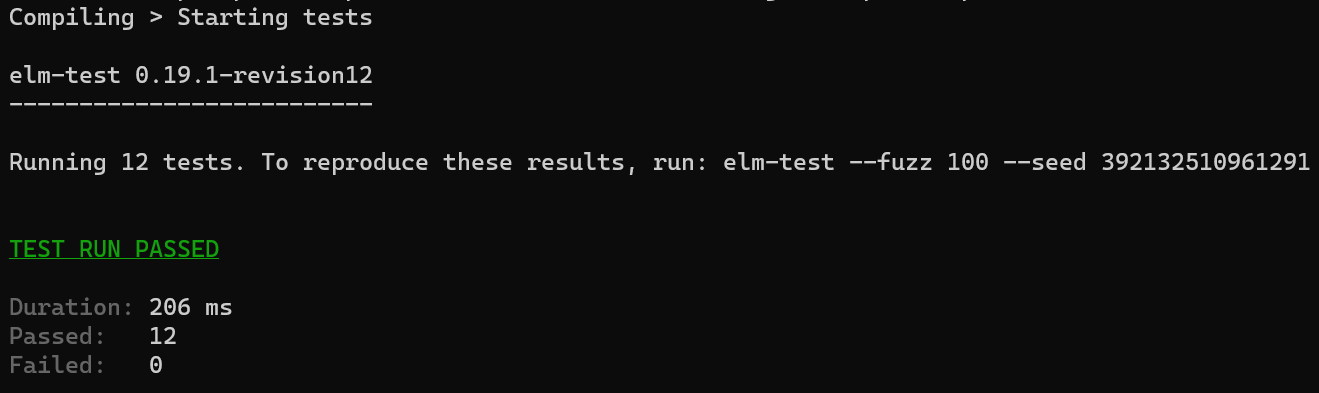
\includegraphics[width=0.9\textwidth]{elmpass.png}
  \caption{Izlaz nakon uspešnog izvršavanja testova}
  \label{fig:elmpass}
\end{figure}

\begin{figure}[!ht]
  \centering
  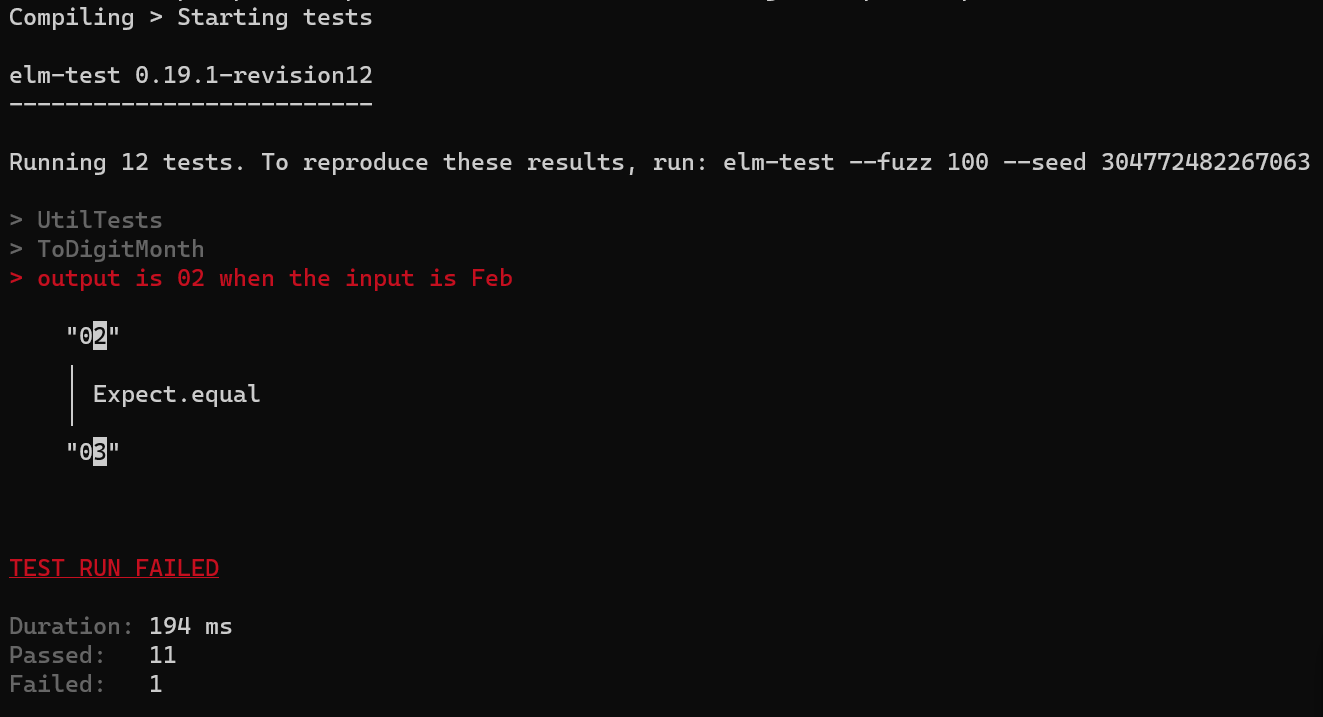
\includegraphics[width=0.9\textwidth]{elmfail.png}
  \caption{Izlaz nakon neuspešnog izvršavanja testova}
  \label{fig:elmfail}
\end{figure}

\par Što se tiče testiranja neispravnog ulaza, anotacija funkcije \emph{toTwoDigitMonth} to ne dozvoljava. Funkcija očekuje kao ulaz vrednost tipa \emph{Month}, koji dolazi iz modula \emph{Time}, a kao izlaz vrednost tipa \emph{String}. U ovakvim uslovima, u testu nije moguće pozvati funkciju sa bilo kojim ulazom koji nije \emph{Month}, jer će Elm kompilator to videti kao grešku i dati odgovarajuće objašnjenje. Kako bi se proširili slučajevi ispravne upotrebe ovakve funkcije, ona se može izmeniti tako da povratna vrednost bude tipa \emph{Maybe String}. Tada, pri prosleđivanju bilo čega što nije jedan od 12 mogućih ispravnih ulaza (po jedan za svaki mesec), funkcija bi vraćala \emph{Nothing}.
\par Funkcija \emph{toTwoDigitMonth} je dobar kandidat za jednostavne testove, kao što su oni iz primera \ref{lst:example}. U programskom jeziku \emph{Elm} ti testovi nazivaju se jedinični testovi i tako će biti nazivani u nastavku ovog poglavlja. Ovakvi testovi pišu se kada je potrebno proveriti specifičan scenario, kao što je neki granični slučaj. Jedinični testovi pozivaju k$\hat{o}$d koji se testira samo jednom, sa odgovarajućim ulazom, i proveravaju da li je izlaz jednak očekivanom. Na primeru ove funkcije, postoji samo 12 mogućih ulaza, pa je zbog toga za testiranje ove funkcije napisano 12 jediničnih testova. 

\subsection{Faz testiranje}
\par Kada postoji jako veliki broj mogućih ulaza, bilo bi nemoguće ostvariti odgovarajuću pokrivenost samo jediničnim testovima. Prednost testiranja u Elm-u je u tome što se mogu kombinovati različite vrste testova kako bi se postigla dobra pokrivenost koda. Pored testova jedinica koda, Elm nudi još jednu vrstu testova --- faz testove. Faz testiranje (eng. \emph{fuzz testing}) je način testiranja u kome se isti test ponavlja iznova sa nasumično generisanim ulazima. Funkcije koje mogu imati veliki broj različitih ulaza predstavljaju dobre kandidate za faz testiranje. Unutar jednog \emph{describe} bloka, mogu se kombinovati jedinični i faz testovi.
\par Funkcija \emph{intToMonth}, delimično prikazana u primeru koda \ref{lst:primerfaz} vrši jednostavno prevođenje celog broja koji predstavlja redni broj meseca u vrednosti tipa \emph{Maybe Month}. U slučaju da je prosleđen broj između 1 i 12, njena povratna vrednost biće konkretan mesec, a za bilo koji drugi ulaz vratiće \emph{Nothing}.

\begin{lstlisting}[language=elm, caption={Implementacija funkcije \emph{intToMonth}},captionpos=b, label={lst:primerfaz}]
intToMonth : Int -> Maybe Month
intToMonth month =
    case month of
     .... 
        12 ->
            Just Dec
        _ ->
            Nothing
\end{lstlisting}

\par Za konkretne ulaze koji će vratiti mesec, napisano je 12 jediničnih testova. Što se tiče poslednjeg slučaja, kada se očekuje izlaz tipa \emph{Nothing}, koristi se faz testiranje. Primer jednostavnog faz testiranja prikazan je u kodu \ref{lst:faztest}. Funkcija \emph{fuzz} je slična funkciji \emph{test}, ali prihvata i dodatni argument --- fazer (eng. \emph{fuzzer}). Uloga fazera je da generiše nasumične vrednosti datog tipa. Unutar modula \emph{Fuzz} postoje fazeri za najčešće korišćene tipove podataka, kao što su \emph{int, float, string, i list} \cite{fuzz}. Ako se koristi fazer za cele brojeve, on će u opštem slučaju generisati 100 vrednosti u intervalu [-50, 50]. U tom intervalu se nalazi i 0, koja je jedan od najčešćih graničnih slučajeva kada su u pitanju celi brojevi. U ovom slučaju, iskorišćen je fazer \emph{intRange} kome se prosleđuje konkretan interval celih brojeva iz koga će se uzimati vrednosti. Napisana su dva faz testa, od kojih jedan proverava ulaze iz intervala [-50, 0], a drugi iz intervala [13, 50]. Još jedna razlika u odnosu na jedinične testove jeste što se anonimnoj funkciji prosleđuje pravi parametar (\emph{month} u ovom primeru) koji se koristi u samom testu. 

\begin{lstlisting}[language=elm, caption={Implementacija faz testova za funkciju \emph{intToMonth}},captionpos=b, label={lst:faztest}]
intToMonthTests =
        describe "intToMonth"
        [  ...
        fuzz (intRange -50 0) "output is Nothing if invalid input" <|
        \month -> intToMonth month
              |> Expect.equal Nothing, 
        fuzz (intRange 13 50) "output is Nothing if invalid input" <|
        \month -> intToMonth month
              |> Expect.equal Nothing
        ]
\end{lstlisting}

\par Modul \emph{Fuzzer} omogućava i kreiranje specifičnih fazera za tipove koji su eksplicitno kreirani. Fazeri dolaze iz ovog modula, ali funkcija \emph{fuzz} potiče iz modula \emph{Test} \cite{testmodul}. U tabeli \ref{tab:fuzzer} prikazane su tri često korišćene faz funkcije iz ovog modula i njihovi opisi.

\begin{table}[!htbp]
\centering
\caption{Funkcije modula \emph{Test} za faz testiranje}
\label{tab:fuzzer}
\begin{center}
\begin{tabular}{ | m{10cm} | m{10em} | } 
 \hline
\textbf{Funkcija} &  \textbf{Opis funkcije} \\ 
  \hline
 \small{\textbf{fuzz2 : Fuzzer a -> Fuzzer b -> String -> (a -> b -> Expectation) -> Test}} & \small{Slično kao \emph{fuzz}, ali prihvata dva fazera i kreira dve nasumične vrednosti, za testiranje funkcija koje imaju dva argumenta.} \\ 
  \hline
   \small{\textbf{fuzz3 :
    Fuzzer a
    -> Fuzzer b
    -> Fuzzer c
    -> String
    -> (a -> b -> c -> Expectation)
    -> Test}} & \small{Slično kao \emph{fuzz}, ali prihvata tri fazera i kreira tri nasumične vrednosti, za testiranje funkcija koje imaju tri argumenta.} \\ 
  \hline
 \small{\textbf{fuzzWith : FuzzOptions a -> Fuzzer a -> String -> (a -> Expectation) -> Test}} & \small{Kreira faz test sa datim opcijama, koje mogu biti broj faz testova (\textit{runs}), ili statistička distrubucija testova (\textit{distribution}).}  \\ 
\hline

\end{tabular}
\end{center}
\end{table}

\par Nakon pokretanja faz testova, na izlazu će se pojaviti seme nasumičnosti koje se može iskoristiti za rekreiranje konkretnih faz testova navođenjem komande \textbf{--seed} iz terminala, a može se i specifikovati konkretan broj faz testova koji će se izvršiti uz komandu \textbf{--fuzz}. Ako neki od testova izazove grešku, na izlazu će pisati koja od vrednosti je izazvala, a ako ih ima više, izabraće najjednostavniju od njih kako bi se što lakše pronašao uzrok. Navođenje većeg broja faz testova pokriva više ulaza, ali sa druge strane, time se povećava vreme izvršavanja. 
\par Faz testiranje se smatra testiranjem zasnovanom na svojstvima (eng. \emph{property based testing}). Njihova uloga je da utvrde da određeno svojstvo važi za sve ulaze i izlaze. U slučaju funkcije \emph{intToMonth}, to svojstvo glasi: za svaki ulaz koji nije ceo broj između 1 i 12, izlaz uvek mora biti \emph{Nothing}. Za razliku od jediničnih testova koji proveravaju samo jedan konkretan scenario, faz testovi omogućavaju testiranje koda na mnogo višem nivou. Pri pisanju ovih testova, neophodno je dobro razmisliti šta je to što k$\hat{o}$d treba da uradi i pronaći svojstvo koje mora biti zadovoljeno, i zatim u testu proveriti da li to svojstvo važi. Kad god je to moguće, uvek treba koristiti faz testove umesto jediničnih. 

\section{Testiranje rada sa JSON podacima}
\par Kodiranje i dekodiranje JSON podataka izvšava se pomoću modula \emph{Json.Encode} i \emph{Json.Decode} iz paketa \emph{elm/json}. Kada nakon HTTP zahteva server pošalje odgovor u JSON formatu, često je neophodno prevesti taj odgovor u odgovarajući slog. Funkcije koje vrše ovo prevođenje nazivaju se dekoderi. U primeru koda \ref{lst:decoderprimer} data je funkcija dekodiranja iz modula \emph{Session}, u kome su izdvojene funkcije za prijavljivanje i odjavljivanje korisnika. Funkcija \emph{decodeSession} dekodira svako polje sloga \emph{Session} i tako pruža validaciju podataka pre nego što oni dođu do aplikacije. 

\begin{lstlisting}[language=elm, caption={Implementacija funkcije dekodiranja \emph{decodeSession}},captionpos=b, label={lst:decoderprimer}]
decodeSession : Decoder Session
decodeSession =
    Decode.map5 Session
        (Decode.field "access_token" Decode.string)
        (Decode.field "expires_in" Decode.float)
        (Decode.field "user" decodeUser)
        (Decode.field "semester_id" Decode.int)
        (Decode.maybe (Decode.field "student_info" decodeStudentInfo))
\end{lstlisting}

\par Unutar dekodera mogu se pozivati i drugi dekoderi --- u ovom primeru to su \emph{decodeUser} i \emph{decodeStudentInfo}, čija je uloga u dekodiranju slogova koji predstavljaju korisnika i studenta. Ipravnost dekodera je jedna od retkih stvari za koje sistem tipova u Elm-u ne može pomoći u pronalaženju grešaka. Pre pisanja samih faz testova, definisani su specifični fazeri, za svaki od slogova. Kako više datoteka sa testovima koristi iste fazere, svi oni su implementirani na jednom mestu --- u pomoćnoj datoteci \emph{tests{\textbackslash}FuzzerHelper.elm}. Svaka datoteka sa testovima uključiće ovu datoteku zajedno sa konkretnim neophodnim fazerima. Za kreiranje nasumičnih kombinacija polja sloga \emph{Session}, definisan je \emph{sessionFuzzer}, prikazan u primeru koda \ref{lst:sessionfuzzer}. Funkcija \emph{map5} će mapirati pet polja i za svako od njih kreirati odgovarajući fazer. Svaki od fazera kreiraće veliki broj različitih vrednosti. Na primer, \emph{Fuzz.string} će generisati nasumične niske, ali sa većom verovatnoćom one za koje se često očekuju greške --- prazne, ili jako dugačke ili kratke niske. Za studenta i korisnika takođe su implementirani specifični fazeri.

\begin{lstlisting}[language=elm, caption={Implementacija fazera za slog \emph{Session}},captionpos=b, label={lst:sessionfuzzer}]
sessionFuzzer : Fuzzer Session
sessionFuzzer = 
    Fuzz.map5 Session
        Fuzz.string
        Fuzz.float
        userInfoFuzzer
        (Fuzz.intRange 1 10)
        (Fuzz.maybe studentInfoFuzzer)
\end{lstlisting} 

\par Fazer je sada spreman za upotrebu iz modula \emph{SessionTests}. Svaki od dekodera istestiran je pojedinačno, a faz testovi koji proveravaju ispravnost funkcije \emph{decodeSession} prikazani su u primeru koda \ref{lst:testdecode}. Priprema testa podrazumeva enkodiranje svakog od polja, koje funkcioniše na sličan način kao i dekodiranje, samo u suprotnom smeru. Enkoderi se takođe mogu kreirati za specifične tipove podataka. Nakon što se objekat enkodira u JSON vrednost, poziva se funkcija \emph{decodeValue} koja prihvata dekoder koji se testira kao prvi argument, i enkodirani objekat kao drugi. Ako je izvršavanje uspešno, očekuje se izlaz oblika \emph{(Ok \_)}, za čiju proveru je zadužena pomoćna funkcija \emph{success}. 
\par U drugom faz testu prikazano je kako se može izvući specifično polje iz rezultata, korišćenjem \emph{Result.map}. Taj test proverava da li će polje \emph{studentInfo} imati očekivanu vrednost \emph{Nothing} ako se u ulazu enkodira \emph{null} na njegovom mestu, s obzirom na to da mu je tip \emph{Maybe}. Ovaj test odnosiće se samo na jedno konkretno polje, umesto na čitavu strukturu. To osigurava da neće biti potrebne manuelne ispravke ovog testa ako se u kodu dese neke izmene, kao na primer dodavanje novog polja. Zbog toga se preporučuje pisanje ovakvih testova koji se fokusiraju na jednu konkretnu stvar i tako sužavaju opseg testa. Takođe, ako se dese greške u nekim drugim poljima, ovaj test će i dalje prolaziti jer nije vezan za ta konkretna polja, i time će olakšati posao pronalaženja greške.

\begin{lstlisting}[language=elm, caption={Implementacija testova za funkciju \emph{decodeSession}},captionpos=b, label={lst:testdecode}]
decodeSessionTests = 
    describe "Session decoder"
    [fuzz sessionFuzzer "fuzz test for decoding session" <| 
     \session -> 
        [("access_token", Encode.string session.accessToken),
         ("expires_in", Encode.float session.expiresIn),
          .... 
        ]
        |> Encode.object
        |> Decode.decodeValue Session.decodeSession
        |> success
        |> Expect.equal True, 
         
     fuzz sessionFuzzer "decoding session with no student info, field should be Nothing" <| 
     \session -> 
        [ ...
         ("student_info", Encode.null)
        ]
        |> Encode.object
        |> Decode.decodeValue Session.decodeSession
        |> Result.map (\s -> s.studentInfo)
        |> Expect.equal (Ok Nothing)
    ]
\end{lstlisting}

\par U slučaju neispravnog ulaza, dekoderi će vratiti rezultat tipa \emph{(Err, \_)}. Kada se to desi, pomoćna funkcija \emph{success} vratiće \emph{False}. Primer jediničnog testa koji proverava neispravan ulaz dat je u kodu \ref{lst:errordecoder}, gde se testira dekoder sloga \emph{Topic}. U testu se priprema ulaz koji je neispravan --- polju \emph{number} dodeli se niska umesto celog broja, zatim se prosledi funkciji i na kraju proveri da li je to dovelo do greške. \emph{Expect.err} radi upravo to, a isto se može postići i upotrebom već spomenute funkcije \emph{success}.

\begin{lstlisting}[language=elm, caption={Implementacija testa koji izaziva grešku na primeru funkcije \emph{Topic.decoder}},captionpos=b, label={lst:errordecoder}]
test "Given invalid input returns (Err _)" <|
      \_ -> 
        let input = """
                { "id" : 1,
                  "title" : "naslov",
                  "number" : "1"} 
            """
             decodedOutput = decodeString Topic.decoder input
        in 
          Expect.err decodedOutput
\end{lstlisting}


\section{Testiranje Arhitekture Elm}
\par U delu \ref{sec:arhitektura} objašnjen je \emph{MVU} obrazac projektovanja koji svaki Elm program implementira. Glavne funkcije koje se nalaze u svakom od modula su funkcije \textbf{\emph{update}} i \emph{\textbf{view}}. U ovoj sekciji, najpre će biiti prikazano testiranje funkcija ažuriranja \emph{update}, čija je uloga da na osnovu primljene poruke od pretraživača kreiraju novi model. Nakon toga, napisani su testovi za funkcije pogleda \emph{view}, na osnovu kojih se generiše HTML.

\subsection{Testiranje promena stanja aplikacije}

\par Celokupno stanje Elm aplikacije predstavljeno je jednom vrednošću modela. Model aplikacije definisan je u datoteci \emph{Main.elm}. \emph{Model} se menja tako što funkcija\emph{update} prihvati poruku \emph{Msg} i kao rezultat izvršavanja vrati novi \emph{Model}. Anotacija funkcije \emph{update} prikazana je u kodu \ref{lst:updateanotacija}. Povratna vrednost je torka modela i komande.  Komande u Elm-u predstavljaju vrednosti koje opisuju operacije koje okruženje Elm treba da izvrši, a koje se ne mogu predstaviti funkcijama. Funkcija \emph{update} predstavlja centralno mesto izvršavanja komandi. \emph{Msg} se odnosi na tip poruke koja se vraća aplikaciji. 

\begin{lstlisting}[language=elm, caption={Anotacija funkcije \emph{update}},captionpos=b, label={lst:updateanotacija}]
update : Msg -> Model -> ( Model, Cmd Msg)
\end{lstlisting}

\par Svaka promena stanja aplikacije može se testirati tako što se u testovima proslede odgovarajuća poruka i model kao argumenti funkcije \emph{update}, i zatim ispita dobijeni model. Svaka stranica koja ima svoj modul ima definisan model, poruke i funkcije \emph{update} i \emph{view} koje se pozivaju iz glavnog modula aplikacije. Sve poruke objedinjuju se u modulu \emph{Main} u jedan glavni tip poruke, a unutar funkcije \emph{update} glavnog modula se na osnovu poruke poziva funkcija \emph{update} odgovarajuće stranice. Trenutni model se ažurira novim modelom date stranice, a poruku komande je potrebno transformisati u odgovarajući glavni tip poruke.
\par U okviru modula \emph{LoginPage.elm}, definisana je funkcija \emph{update} prikazana u kodu \ref{lst:loginupdate}. Na osnovu vrste poruke koja se prosledi, model se menja na određeni način. Na primer, kada se prosledi tip poruke \emph{Email}, desiće se jednostavna izmena stanja --- ažuriraće se polje \emph{email}.

\begin{lstlisting}[language=elm, caption={Funkcija \emph{update} stranice za prijavljivanje korisnika \emph{LoginPage}},captionpos=b, label={lst:loginupdate}]
update : Msg -> Model -> ( Model, Cmd Session.Msg )
update msg model =
    case msg of
        Email email ->
            ( { model | email = email }, Cmd.none )
       .... 
        SubmittedForm ->
            ({model | error = Nothing, processing = True}, getSession {email = model.email, password = model.password, apiBaseUrl = model.apiBaseUrl})
\end{lstlisting}

\par Testovi ove funkcije prikazani su u primeru koda \ref{lst:loginupdatetest}. Napisan je po jedan faz test za svaki od tipova poruka. Kreira se fazer za model i zatim se nad njim pozove funkcija ažuriranja. Pomoću \emph{Tuple.first} dohvati se samo prvi član torke iz rezultata, koji predstavlja model. Na kraju se proveri da li polje ima odgovarajuću vrednost. Kada je u pitanju drugi deo povratne vrednosti (\emph{Cmd msg}), Elm još uvek nema mogućnost za ispitivanje \emph{Cmd} vrednosti kako bi se utvrdilo koju komandu predstavlja. Jedan od načina da se to postigne jeste da se testiraju podaci pre nego što se pretvore u komandu. Umesto direktnog testiranja komandi, testiraju se funkcije koje kreiraju te vrednosti. U ovom primeru to je funkcija \emph{getSession}. Ideja je da se funkcija oblika \emph{getCmd : Foo -> Cmd Msg} podeli na dve funkcije kako bi se olakšalo testiranje: 

\begin{enumerate}
\item \emph{getData : Foo -> FooData} --- funkcija koja se testira
\item \emph{sendFooData : FooData -> Cmd Msg} --- jednostavna funkcija koja se ne testira 
\end{enumerate}

\par Jedan od alternativnih načina testiranja komandi je da se kreira specijalan tip koji će predstavljati sve moguće komande aplikacije i postaviti ga kao povratnu vrednost funkcije \emph{update}. Pored toga, napisati funkciju koja prevodi taj tip u \emph{Cmd Msg}. Na taj način će povratna vrednost biti nešto što se može do detalja ispitati. Iako korisna, ova tehnika se retko koristi, i najčešće se jednostavno preskoči testiranje samih komandi. Postoji još korisnih tehnika koje ovde neće biti spominjane jer zahtevaju značajne izmene originalnog koda \cite{cmd1, cmd2}. 

\begin{lstlisting}[language=elm, caption={Testovi za funkciju \emph{update} modula \emph{LoginPage}},captionpos=b, label={lst:loginupdatetest}]
    [fuzz2 string loginModelFuzzer "Email msg sets the email" <|
    \email model -> 
        model
        |> update (Email email)
        |> Tuple.first 
        |> .email 
        |> Expect.equal email,
    ...
\end{lstlisting}


\subsection{Testiranje HTML sadržaja}

\par Nakon što funkcija ažuriranja kreira model, on se prosleđuje funkciji \emph{view}, koja taj model transformiše u HTML koji će se prikazati korisniku. Ona prihvata model kao ulaz, a njena povratna vrednost ima tip html poruke. Anotacija svake funkcije \emph{view} je ista i data je u kodu \ref{lst:viewanot}.

\begin{lstlisting}[language=elm, caption={Anotacija funkcije \emph{view}},captionpos=b, label={lst:viewanot}]
view : Model -> Html Msg
\end{lstlisting}

\par Za kreiranje HTML čvorova i atributa koriste se funkcije iz modula \emph{Html}. Za opisivanje izgleda stranice u ovom projektu korišćene su funkcije modula \emph{Html.Styled}. Stilizovanje HTML elemenata bez upotrebe css datoteka omogućeno je pomoću paketa \emph{NoRedInk/noredinkui}. U primeru koda \ref{lst:loginview} prikazana je funkcija pogleda za stranicu prijavaljivanja korisnika. Funkcije koje pruža modul \emph{Html}, koje služe za kreiranje čvorova i atributa, imaju nazive po HTML oznakama (\emph{node}, \emph{button} itd.) i tako omogućavaju bolju čitljivost koda. U ovom primeru, navode se jednostavni elementi kao što su zaglavlja, polja za unos imejl adrese i šifre, i jedno dugme koje aktivira događaj. 

\begin{lstlisting}[language=elm, caption={Funkcija \emph{view} modula \emph{LoginPage}},captionpos=b, label={lst:loginview}]
view model =
    Container.view
  	...
            [ Heading.h3 [ Heading.css [ marginBottom (px 20) ] ] [ Html.text "Prijava korisnika" ]
            	... 
            , Button.button "Prijavi se"
                [  ... , Button.onClick SubmittedForm ]
            ]
        ]
\end{lstlisting}

\par Testiranje funkcija pogleda podrazumeva ispitivanje konkretnih HTML vrednosti. Pre pisanja testova za funkcije \emph{view} neophodno je uključiti paket \emph{elm-html-test} \cite{html-elm-test}. Ovaj paket omogućava kreiranje očekivanja o HTML vrednostima, i zbog toga je njegova glavna namena testiranje funkcija pogleda. Unutar njega, postoje tri najvažnija podmodula namenjena za testiranje različitih svojstava koje funkcija \emph{view} generiše:

\begin{enumerate}
\item \textbf{\emph{Test.Html.Query}} --- omogućava pisanje upita nad HTML strukturama
\item \textbf{\emph{Test.Html.Event}} --- omogućava simuliranje događaja nad HTML vrednostima
\item \textbf{\emph{Test.Html.Selector}} --- omogućava dohvatanje HTML elemenata
\end{enumerate}

\par Pri testiranju pogleda neophodno je razmisliti šta konkretno testirati. Ne preporučuje se testiranje doslovnog izlaza, jer to izaziva visoku spregnutost između testa i implementacije samog koda. Na primer, ako se dese sitne izmene u svrhu stilizovanja stranice, to bi dovelo do padanja testa koji doslovno proverava prisutne elemente. Ono što treba testirati jeste neka važna logika koju funkcija implementira. Ako neka funkcija \emph{view} prikazuje odgovarajući tekst u zavisnosti od određenog polja modela, to je nešto što je vredno testiranja. Kako bi se predstavili osnovni koncepti modula \emph{Test.Html.Query}, u primeru koda \ref{lst:viewtest} prikazan je jednostavan test koji proverava prisustvo očekivanog teksta pri prikazivanju stranice za prijavljivanje korisnika. U svakom testu funkcija pogleda, nad rezultatom pozivanja funkcije sa datim modelom prvo se poziva funkcija \emph{Query.fromHtml}. Njena uloga je da prihvati HTML i vrati vrednost tipa \emph{Single}, koja predstavlja koreni čvor HTML-a. U ovom slučaju to je glavni kontejner u kome su sadržani svi elementi sa stranice. Nakon toga, upotrebljena je funkcija \emph{Query.has} koja proverava da li se prosleđeni element sadrži sve što mu je dato u listi selektora. U ovoj listi prosleđen je selektor \emph{text} iz modula \emph{Html.Selector}, koji treba da se poklopi sa svim elementima koji sadrže atribut \emph{text} sa datom vrednošću. Ova funkcija vraća vrednost tipa \emph{Expectation}, što znači da se može naći na kraju cevovoda u testu. Slično kao sa tekstom, može se proveriti prisustvo dugmadi, polja za unos teksta i drugih HTML elemenata. Funkcije kao što su \emph{find}, \emph{findAll, contains, count} iz modula \emph{Html.Query}, i \emph{tag, containing, attribute} iz modula \emph{Html.Selector}, su neke od tih koje omogućavaju takve provere.

\begin{lstlisting}[language=elm, caption={Test za funkciju \emph{view} modula \emph{LoginPage}},captionpos=b, label={lst:viewtest}]
    [fuzz loginModelFuzzer "Correctly renders text in DOM" <|
     \model ->
        model
        |> LoginPage.view 
        |> Html.toUnstyled
        |> Query.fromHtml
        |> Query.has [ text "Prijava korisnika" ]
\end{lstlisting}


\subsubsection{Testiranje interakcija sa korisnikom}

\par Kada je utvrđeno da se na stranici prikazuje sve što je očekivano, može se preći na testiranje ispravnosti odgovarajućih događaja --- na primer, da li se k$\hat{o}$d ponaša očekivano kada se klikne na dugme. Na primeru prijave korisnika, klikom na dugme sa tekstom \emph{''Prijavi se''} funkciji \emph{update} se prosleđuje poruka tipa \emph{SubmittedForm}, koja dalje poziva druge funkcije koje će izvršiti \emph{post} zahtev. Pomoću modula \emph{Html.Test.Event} simulira se događaj klika na dugme u testu. Deo testa prikazan je u kodu \ref{lst:eventtest}. Najpre se pronađe dugme pomoću upita i selektora koji proverava da li dugme sadrži tekst ''Prijavi se'', a zatim se nad njim simulira događaj klika pozivom funkcije \emph{Event.simulate}, za koji se očekuje da će vratiti poruku tipa \emph{SubmittedForm}. 
\par Drugi tip događaja simuliran u ovom modulu je događaj unosa teksta u polja namenjena za imejl adresu i šifru korisnika. Sintaksa je slična i koristi se funkcija \emph{Event.input} koja prihvata nisku koja se unosi. Unosom teksta ažuriraju se odgovarajuća polja modela. Primer ovog testa dat je u kodu \ref{lst:eventinputtest}. 

\begin{lstlisting}[language=elm, caption={Simulacija događaja klika na dugme u testu funkcije \emph{view} modula \emph{LoginPage}},captionpos=b, label={lst:eventtest}]
LoginPage.view model
	  ... 
            |> Query.find
                [ tag "button"
                , containing [ text "Prijavi se" ]
                ]
            |> Event.simulate Event.click
            |> Event.expect SubmittedForm
\end{lstlisting}

\begin{lstlisting}[language=elm, caption={Simulacija događaja unosa teksta u testu funkcije \emph{view} modula \emph{LoginPage}},captionpos=b, label={lst:eventinputtest}]
        |> Query.fromHtml
        |> Query.find [ attribute <| Attributes.placeholder "Email" ]
        |> Event.simulate (Event.input emailString)
        |> Event.expect (Email emailString)
\end{lstlisting}


%\chapter{Testiranje celokupnog sistema --- End to End}
%\label{chp:e2e}

%\section{Integracija klijentske i serverske strane}

%\section{Testiranje opterećenja}

% ------------------------------------------------------------------------------
\chapter{Zaključak}
% ------------------------------------------------------------------------------
% TODO spomunitu semaphore
% TODO moglo bi da se doda jos obrada gresaka, tipa ako je age vece od 100 onda Err '''cant be that old'''
%TODO making impossible staes impossible
% ------------------------------------------------------------------------------
% Literatura
% ------------------------------------------------------------------------------
\literatura

% ==============================================================================
% Završni deo teze i prilozi
\backmatter
% ==============================================================================

% ------------------------------------------------------------------------------
% Biografija kandidata
%\begin{biografija}

%\end{biografija}
% ------------------------------------------------------------------------------

\end{document}
